
\documentclass[11pt,a4paper]{article}

\usepackage[margin=2.5cm]{geometry}
\usepackage{amsmath}
\usepackage{graphicx}
\usepackage{booktabs}
\usepackage{float}
\usepackage{hyperref}
% Improved academic report formatting
\usepackage{lmodern}
\usepackage{microtype}
\usepackage{setspace}
\usepackage{titlesec}
\usepackage{subcaption}

\titlespacing*{\section}{0pt}{12pt}{2pt}
\titlespacing*{\subsection}{0pt}{6pt}{4pt}

\setstretch{1.12}
\setlength{\parindent}{0pt}
\setlength{\parskip}{6pt}
\setlength{\abovedisplayskip}{6pt}
\setlength{\belowdisplayskip}{6pt}

\title{Exploratory Statistical Analysis of
Amazon Data Science Books}

\author{
Florentia Pattidou \and
Valeria Shirshina \and
Marios Makrygiannis
}

\date{University of Cyprus\\
DSC531 -- Statistical Simulation and Analysis}

\begin{document}
\maketitle
\newpage
\begin{abstract}
This report presents an exploratory statistical analysis of the Amazon Data Science Books dataset using the R programming language. The objective is to examine the characteristics of data science books, assess data quality, summarize key numerical variables, and investigate relationships between book attributes and customer reviews. 

The original dataset contains 946 observations and 11 variables. During data cleaning, one duplicate observation was removed, missing values were examined, and book weights were converted into kilograms. Potential outliers were investigated using the interquartile range (IQR) method and additional weight-per-page checks. Ten potentially suspicious weight measurements were flagged for a separate sensitivity analysis without removing the corresponding books.

Descriptive statistics and graphical methods were used to explore the distributions of prices, page counts, ratings, review counts, and weights. The results indicate that review counts are highly right-skewed, while average customer ratings are generally concentrated toward the upper end of the rating scale. A moderate positive correlation was observed between page counts and prices (r = 0.444).

Overall, the analysis demonstrates how data cleaning, descriptive statistics, and visualization can support the interpretation of real-world book data.

\end{abstract}
\newpage
\tableofcontents
\newpage
\section{Introduction}
Data analysis plays an important role in understanding patterns, identifying relationships, and extracting meaningful insights from real-world datasets. Statistical methods allow researchers to summarize large amounts of information, evaluate variability, and investigate potential associations between variables.

This report presents an exploratory statistical analysis of the Amazon Data Science Books dataset using the R programming language. The dataset contains information about books related to data science, including their prices, number of pages, average customer ratings, number of reviews, rating distributions, and physical weights.

The primary objective of this study is to examine the characteristics of the dataset through data cleaning, descriptive statistics, and graphical visualization. Particular attention is given to identifying missing values, duplicate observations, potentially unusual measurements, and patterns within the numerical variables.

Additionally, the analysis investigates relationships between selected book characteristics, such as the association between the number of pages and price, the relationship between pages and physical weight, and the connection between customer ratings and review counts.

By combining statistical summaries with visual representations, this study aims to provide a clearer understanding of the dataset and demonstrate how exploratory data analysis can support informed interpretation of real-world information.
\newpage
\section{Dataset Description}
\begingroup
\setlength{\parskip}{3pt}
\renewcommand{\arraystretch}{0.9}
\subsection{Dataset Overview}
The Amazon Data Science Books dataset contains 946 observations
and 11 variables describing book characteristics and customer
feedback. These include prices, page counts, customer ratings,
review counts, star-rating proportions, weights, and languages.

The dataset was imported into R using \texttt{read.csv()}
and initially examined using \texttt{dim()}, \texttt{str()},
and \texttt{summary()}. This examination identified missing
values and inconsistent weight units, which were addressed
during data cleaning.
\subsection{Description of Variables}
Table~\ref{tab:variables} presents the variables included
in the original dataset, their data types, and their meanings.
\begin{table}[H]
\centering
\small
\begin{tabular}{lll}
\toprule
Variable & Data Type & Description \\
\midrule
\texttt{price} & Numeric & Book price \\
\texttt{pages} & Integer & Number of pages \\
\texttt{avg\_reviews} & Numeric & Average customer rating (1--5) \\
\texttt{n\_reviews} & Integer & Number of customer reviews \\
\texttt{star5} & Numeric & Proportion of five-star ratings \\
\texttt{star4} & Numeric & Proportion of four-star ratings \\
\texttt{star3} & Numeric & Proportion of three-star ratings \\
\texttt{star2} & Numeric & Proportion of two-star ratings \\
\texttt{star1} & Numeric & Proportion of one-star ratings \\
\texttt{weight} & Character & Book weight in ounces or pounds \\
\texttt{language} & Character & Language of the book \\
\bottomrule
\end{tabular}
\caption{Description of the Original Dataset Variables}
\label{tab:variables}
\end{table}
The five star-rating variables represent proportions rather
than absolute review counts. The weight variable requires
conversion to a common measurement unit before numerical analysis.
\subsection{Initial Data Quality Assessment}
Table~\ref{tab:missing} summarizes the missing values
identified during the initial inspection of the dataset.

\begin{table}[H]
\centering
\begin{tabular}{lr}
\toprule
Variable & Missing Values \\
\midrule
\texttt{price} & 2 \\
\texttt{pages} & 12 \\
\texttt{avg\_reviews} & 123 \\
\texttt{weight} & 3 blank strings \\
\texttt{language} & 3 blank strings \\
\bottomrule
\end{tabular}
\caption{Initial Missing Values}
\label{tab:missing}
\end{table}
The initial assessment identified missing information
in several variables. Blank strings in the weight and
language fields required conversion to \texttt{NA}.
Missing observations were not automatically removed,
allowing available information to be retained for
subsequent analysis. Duplicate records and potentially
unusual measurements were investigated during the
cleaning process described in Section~\ref{sec:cleaning}.
\section{Data Cleaning}
\label{sec:cleaning}
\subsection{Data Cleaning Overview}

Data cleaning was performed in R to improve data consistency
while preserving as much information as possible. The procedures
included handling missing values, removing duplicate observations,
standardizing weight measurements, investigating outliers,
and validating customer review information.

\subsection{Missing Values and Duplicate Observations}

Blank strings in the weight and language variables were converted
to \texttt{NA}. Missing values were handled using available-case
calculations rather than deleting incomplete observations.
One exact duplicate was identified and removed, reducing the
dataset from 946 to 945 observations.

\subsection{Weight Standardization}

Book weights were originally recorded in two units:
ounces (204 observations) and pounds (738 observations),
with 3 missing measurements. 
The following conversion factors were applied:
\begin{align*}
\text{Ounces to kilograms:}\quad
W_{\mathrm{kg}} &= W_{\mathrm{oz}} \times 0.0283495 \\[8pt]
\text{Pounds to kilograms:}\quad
W_{\mathrm{kg}} &= W_{\mathrm{lb}} \times 0.4535924
\end{align*}

\subsection{Outlier Detection Using the IQR Method}

Potential outliers were identified using the interquartile
range (IQR) method, with boundaries defined as:
\begin{align*}
IQR &= Q_3 - Q_1 \\[6pt]
\text{Lower Bound} &= Q_1 - 1.5 \times IQR \\[6pt]
\text{Upper Bound} &= Q_3 + 1.5 \times IQR
\end{align*}
For book weight, the IQR was approximately 0.448 kg, producing an upper boundary of 1.602 kg. The method identified 41 potential weight outliers. Other variables also contained outliers: price (97), pages (17), average ratings (34), and review counts (111).

These observations were not automatically removed because extreme values may represent genuine book characteristics rather than recording errors.
\newpage
\subsection{Investigation of Suspicious Weight Measurements}
The IQR method identified potential weight outliers, but
these observations were not necessarily incorrect. To investigate unusual weight measurements further, the relationship between book weight and page count was examined.

A weight-per-page ratio was calculated for books with available positive page counts and weight measurements:
\[
\text{Weight per page (g/page)}
=
\frac{1000 \times W_{\mathrm{kg}}}{\text{Pages}}
\]
Measurements outside the exploratory range of
0.3--10 grams per page were flagged as potentially
suspicious. This criterion identified 10 observations.
\begin{table}[H]
\centering
\begin{tabular}{ll}
\toprule
Criterion & Value \\
\midrule
Lower threshold & 0.3 g/page \\
Upper threshold & 10 g/page \\
Flagged observations & 10 \\
\bottomrule
\end{tabular}
\caption{Criteria for Flagging Suspicious Weight Measurements}
\label{tab:weightcriteria}
\end{table}
The flagged measurements were not confirmed data errors.
Therefore, the corresponding books were retained in the
cleaned dataset. For weight-specific sensitivity analysis,
a separate variable, \texttt{weight\_analysis}, was created
by replacing the 10 flagged weight values with \texttt{NA}.

The mean weight decreased from approximately 0.778 kg to
0.753 kg, while the standard deviation decreased from
0.583 kg to 0.404 kg. The Pearson correlation between
page count and weight increased from 0.571 to 0.865.
Because the filtering criterion was based on weight
relative to page count, this increase should be
interpreted cautiously rather than as independent
evidence of a stronger underlying relationship. The corresponding scatterplots are presented in Figure~\ref{fig:pagesweight}.
\begin{figure}[H]
    \centering
    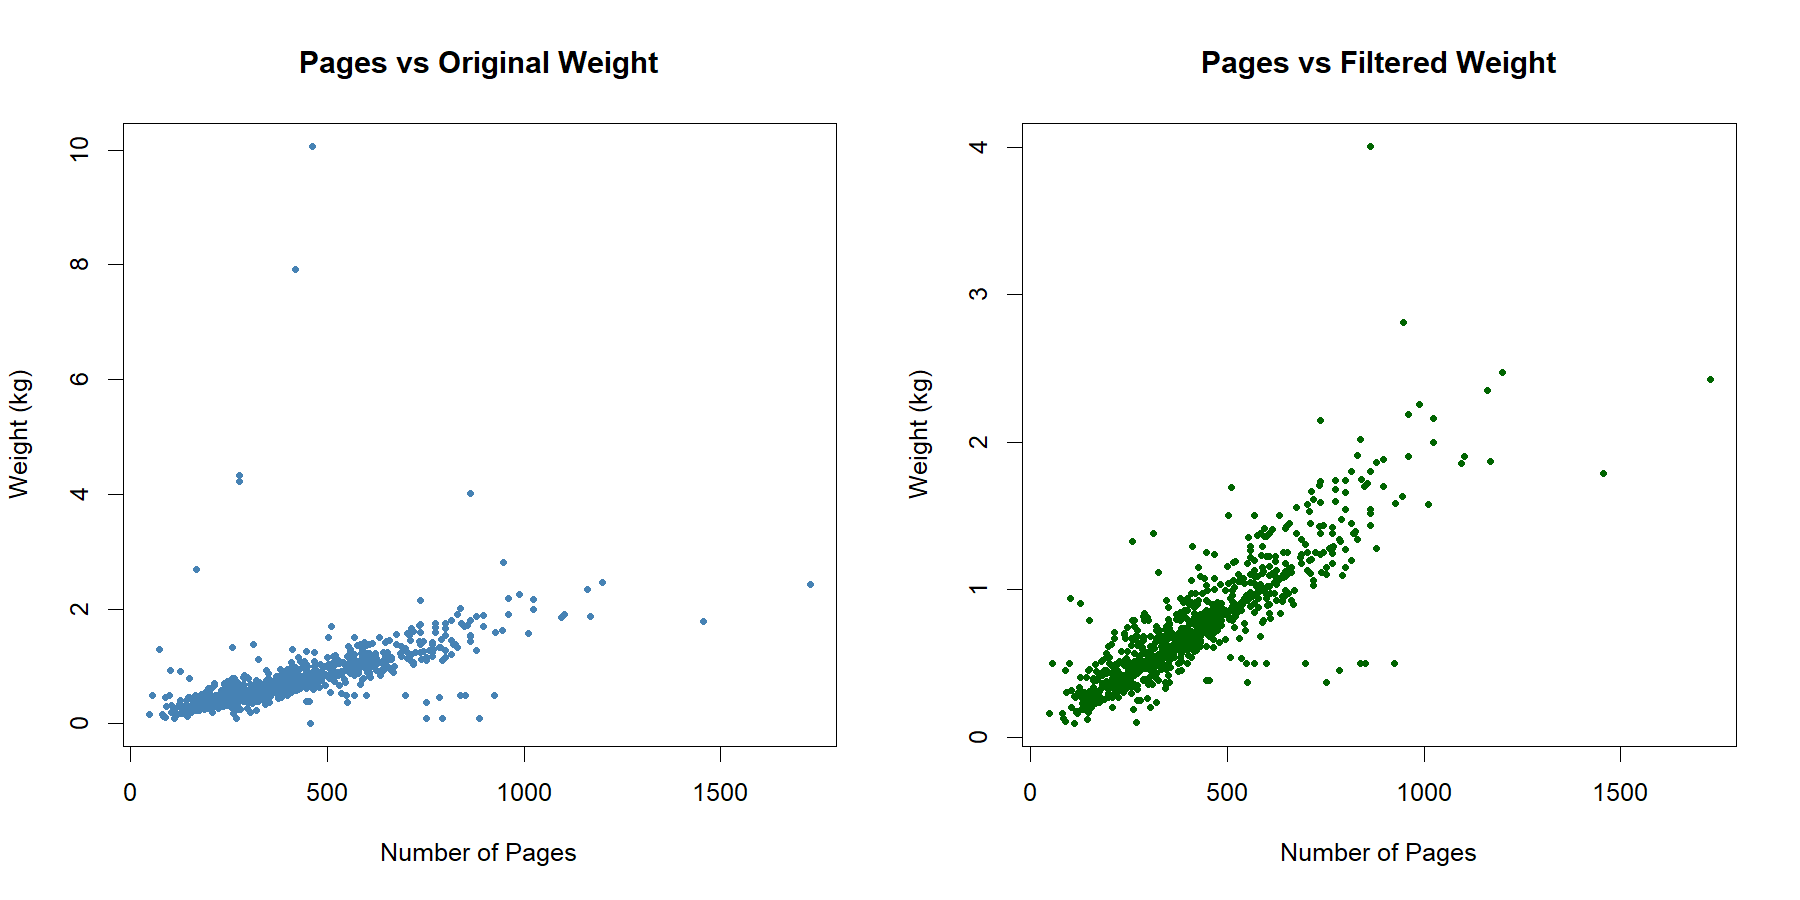
\includegraphics[width=0.85\textwidth]{plots/4_6_pages_vs_weight.png}
    \caption{Relationship Between Page Count and Book Weight Before and After Filtering Suspicious Measurements}
    \label{fig:pagesweight}
\end{figure}

Figure~\ref{fig:pagesweight} compares the relationship
between page count and book weight before and after
excluding the ten flagged measurements from the
weight-specific sensitivity analysis.

The original standardized weight measurements include
all available values, whereas the filtered analysis
excludes potentially suspicious measurements without
removing the corresponding books from the dataset.

Although the filtered data show a stronger positive
correlation, this increase should be interpreted
cautiously because the filtering criterion itself
depends on the weight-to-page ratio.

\subsection{Review Data Consistency}
Customer review information was examined to identify
inconsistencies between review counts, average ratings,
and star-rating proportions.

A total of 123 books had zero customer reviews. For
these observations, the star-rating proportions were
set to \texttt{NA}, since no rating distribution could
be meaningfully calculated.

For the remaining 822 books with customer reviews,
the five star-rating proportions were checked to
determine whether their sum was approximately equal
to one. No observations exceeded a tolerance of
0.05 from the expected total.

These checks helped ensure that the review-related
variables were internally consistent before
subsequent statistical analysis.

\subsection{Final Cleaned Dataset}

After data cleaning, the dataset contained 945 observations,
following the removal of one exact duplicate. Missing values
were preserved as \texttt{NA}, and available weight measurements
were standardized to kilograms.

The cleaned dataset included the original numerical book
characteristics and star-rating proportions, together with
two weight-related variables: \texttt{weight\_kg}, containing
the standardized measurements, and \texttt{weight\_analysis},
used for sensitivity analysis after flagging 10 potentially
suspicious weight values.

\begin{table}[H]
\centering
\begin{tabular}{ll}
\toprule
Characteristic & Final Result \\
\midrule
Original observations & 946 \\
Final observations & 945 \\
Duplicate observations removed & 1 \\
Available weight measurements & 942 \\
Weight values used in sensitivity analysis & 932 \\
Flagged suspicious weights & 10 \\
\bottomrule
\end{tabular}
\caption{Summary of the Final Cleaned Dataset}
\label{tab:cleaned}
\end{table}
The cleaned dataset was exported as a CSV file for
subsequent descriptive statistics and visualization.
No books were removed solely because of extreme values
or missing information.
\newpage
\section{Descriptive Statistics}

\subsection{Summary of Numerical Variables}

Descriptive statistics were calculated for the main numerical
variables, including book prices, page counts, average customer
ratings, review counts, and filtered book weights.

Table~\ref{tab:descriptive} presents the number of available
observations, mean, median, standard deviation, coefficient
of variation (CV), and skewness.

\begin{table}[H]
\centering
\small
\begin{tabular}{lrrrrrr}
\toprule
Variable & N & Mean & Median & SD & CV (\%) & Skewness \\
\midrule
Price & 943 & 52.111 & 43.970 & 36.609 & 70.25 & 2.421 \\
Pages & 933 & 419.478 & 384.000 & 204.060 & 48.65 & 1.123 \\
Average Rating & 822 & 4.441 & 4.500 & 0.401 & 9.03 & -2.011 \\
Number of Reviews & 945 & 137.898 & 25.000 & 499.731 & 362.39 & 9.467 \\
Filtered Weight (kg) & 932 & 0.753 & 0.669 & 0.404 & 53.66 & 1.670 \\
\bottomrule
\end{tabular}
\caption{Descriptive Statistics of the Main Numerical Variables}
\label{tab:descriptive}
\end{table}

The number of available observations differs between variables
because missing values were excluded only from the relevant
calculations. Filtered weight statistics were calculated using
the \texttt{weight\_analysis} variable.
\subsection{Central Tendency and Variability}
The number of customer reviews exhibits the greatest relative
variability (CV = 362.39\%). Its mean (137.898) is considerably
higher than its median (25), indicating that a small number of
highly reviewed books influence the average.

Book prices also exhibit substantial variability (CV = 70.25\%),
while page counts and filtered weights show moderate-to-high
relative variability. In contrast, average customer ratings
have the lowest CV (9.03\%), indicating that ratings are
concentrated within a relatively narrow range.

\subsection{Distribution Shape and Skewness}

Skewness measures the asymmetry of a distribution.
Positive values indicate a longer right tail, while
negative values indicate a longer left tail.

Customer review counts exhibit strong positive skewness
(9.467), indicating that most books receive relatively
few reviews, while a small number receive exceptionally
high counts. Book prices (2.421), page counts (1.123),
and filtered weights (1.670) are also positively skewed.

In contrast, average customer ratings are negatively
skewed (-2.011), reflecting the concentration of ratings
toward the upper end of the five-star scale.

Original book weights had a skewness of 7.209, which
decreased to 1.670 after excluding ten potentially
suspicious measurements from the weight-specific analysis.

Overall, the distributions are asymmetric, highlighting
the importance of using the median and interquartile range
alongside the mean and standard deviation.

\newpage
\section{Data Visualization}

\subsection{Histograms of Numerical Variables}

Histograms were used to examine the distributions of book
prices, page counts, customer review counts, average ratings,
and filtered book weights.

Figure~\ref{fig:histograms} presents the distributions of
these five numerical variables.

\begin{figure}[H]
    \centering
    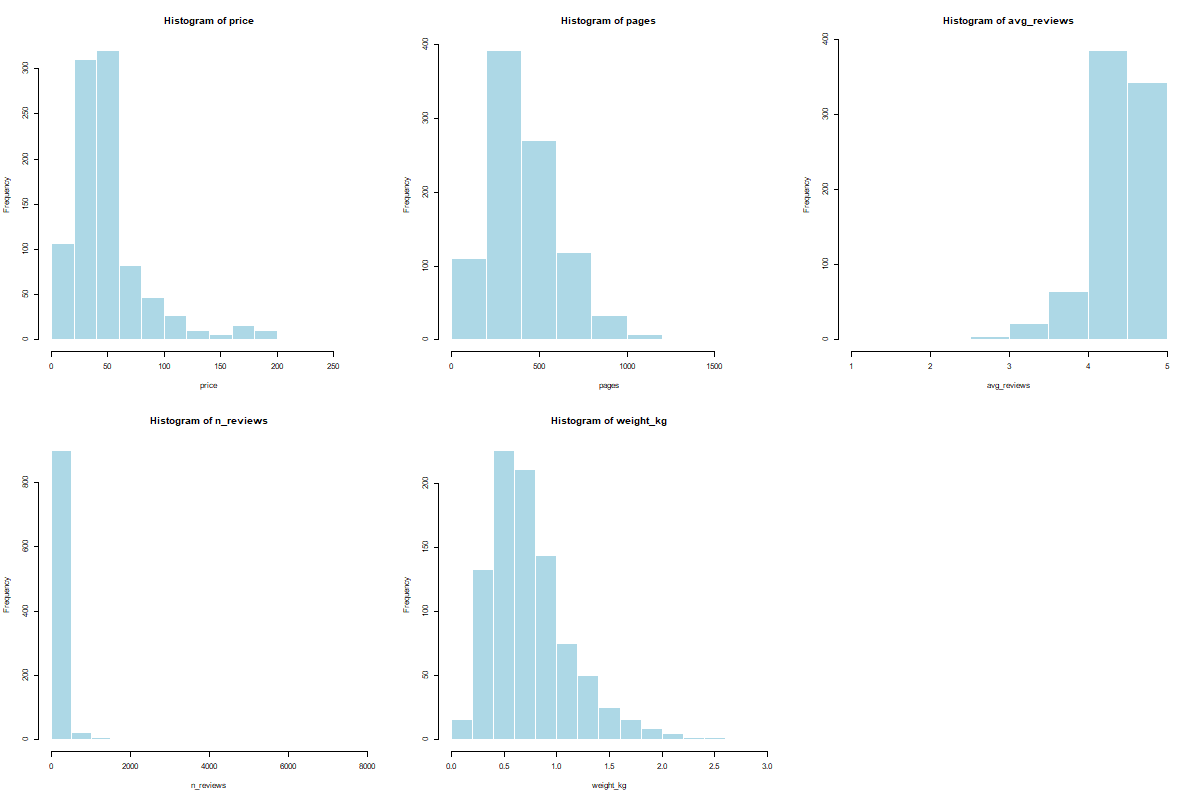
\includegraphics[width=0.95\textwidth]{plots/4_1_histograms.png}
    \caption{Histograms of the Main Numerical Variables}
    \label{fig:histograms}
\end{figure}

The histograms show that book prices, page counts, and
review counts are positively skewed. Review counts exhibit
particularly strong right-skewness, with most books receiving
relatively few reviews and a small number receiving thousands.

Average customer ratings are concentrated toward the upper
end of the five-star scale, while filtered book weights
remain positively skewed. These findings are consistent
with the descriptive statistics presented in Section 4.


More specifically, the distribution of average customer
ratings is negatively skewed, with most observations
concentrated around 4.5 stars.

An additional concentration is visible at the maximum
rating of 5.0, indicating that some books have received
a perfect average customer rating.

This pattern may be influenced by books with relatively
few customer reviews, although the histogram alone
cannot establish the underlying explanation.

The concentration of ratings near the upper boundary
also highlights the bounded nature of the five-star
rating scale.


\subsection{Boxplots and Outlier Visualization}
Boxplots were used to compare the variability of the main
numerical variables and identify observations lying beyond
the typical range of each distribution.

Figure~\ref{fig:boxplots} presents the boxplots of book
prices, page counts, average ratings, review counts,
and filtered book weights.
\begin{figure}[H]
    \centering
    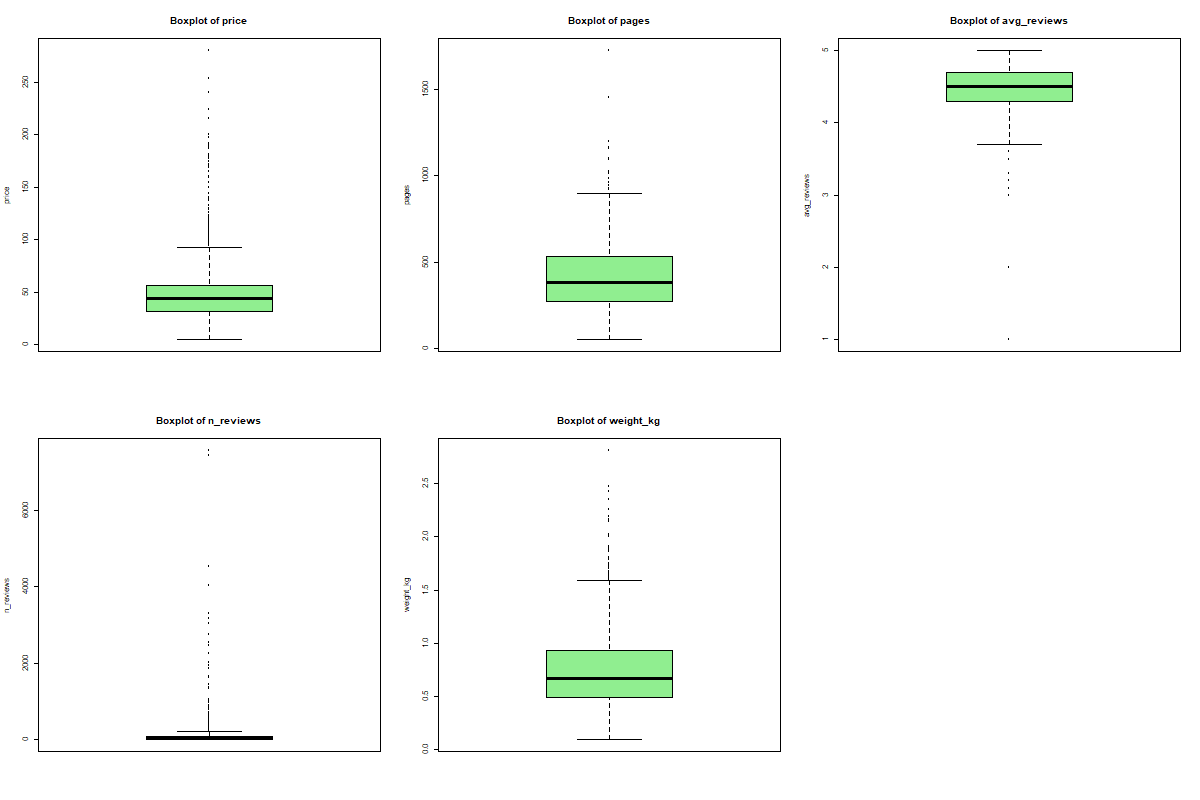
\includegraphics[width=0.95\textwidth]{plots/4_2_boxplots.png}
    \caption{Boxplots of the Main Numerical Variables}
    \label{fig:boxplots}
\end{figure}

The boxplots reveal substantial differences in the spread
of the numerical variables. Review counts exhibit numerous
extreme observations, consistent with their high standard
deviation and coefficient of variation.

Book prices and page counts also contain observations
beyond the upper whiskers, indicating the presence of
relatively expensive and unusually long books.

Average customer ratings are concentrated near the upper
end of the rating scale, with some comparatively low
ratings appearing as outliers. Filtered book weights
still contain high values, even after the ten suspicious
measurements were excluded from the weight-specific analysis.

Overall, these visualizations complement the descriptive
statistics and demonstrate that extreme observations
remain an important characteristic of the dataset.

Observations appearing beyond the boxplot whiskers
are considered potential outliers according to the
1.5 $\times$ IQR rule. However, these values are not
necessarily data errors and were not automatically
removed from the dataset.

\subsection{Log Transformation of Review Counts}

The number of customer reviews exhibited substantial
positive skewness, with a small number of books receiving
exceptionally high review counts.

To examine this distribution more clearly, a logarithmic
transformation was applied:
\[
Y = \log(1 + X)
\]
where $X$ represents the original number of reviews.
Adding one allows books with zero reviews to be included,
since $\log(0)$ is undefined.
Figure~\ref{fig:logreviews} presents the distribution
of log-transformed review counts.
\begin{figure}[H]
    \centering
    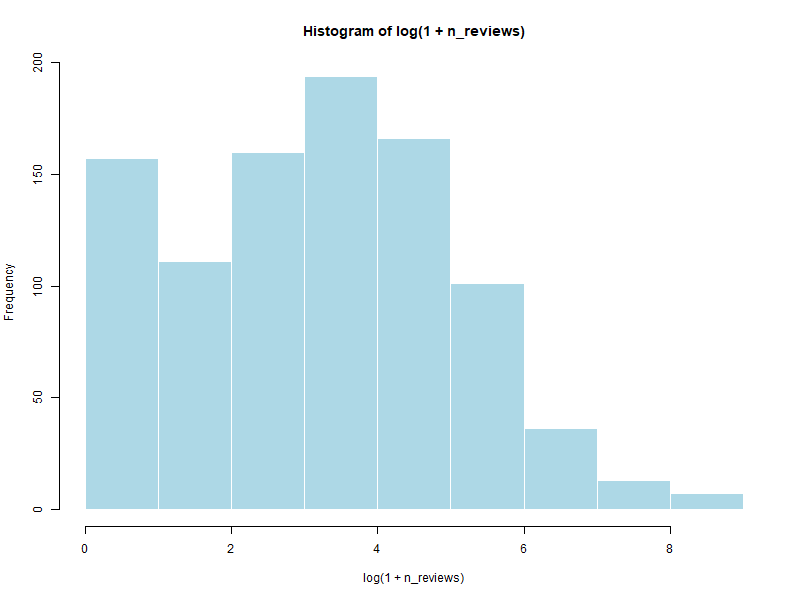
\includegraphics[width=0.85\textwidth]{plots/4_3_log_reviews.png}
    \caption{Histogram of Log-Transformed Review Counts.}
    \label{fig:logreviews}
\end{figure}

The original review-count distribution had a skewness
of 9.467, indicating a strong right tail. Following
the transformation, skewness decreased to approximately
0.055, indicating substantially reduced asymmetry.

The transformation compresses large review counts while
preserving their relative ordering. This makes the
distribution easier to visualize and may be useful for
subsequent statistical analysis. However, low skewness
alone does not establish that the transformed data
follow a normal distribution.
\newpage
\subsection{Log-Transformed Variables and Average Customer Ratings}
First, to analyse the variability of the variables we will construct histograms of all numerical variables. It can be seen that most of the variables are heavily right-skewed. The only variable that is left-skewed is average reviews. So it seems that people tend to leave positive reviews more often than negative ones.

To transform the skewed variables we will use log transformation. All the variables are positive so we will not meet any problems here. Log transformation is an important step which can help for the future model building and hypothesis testing.

\begin{figure}[H]
    \centering
    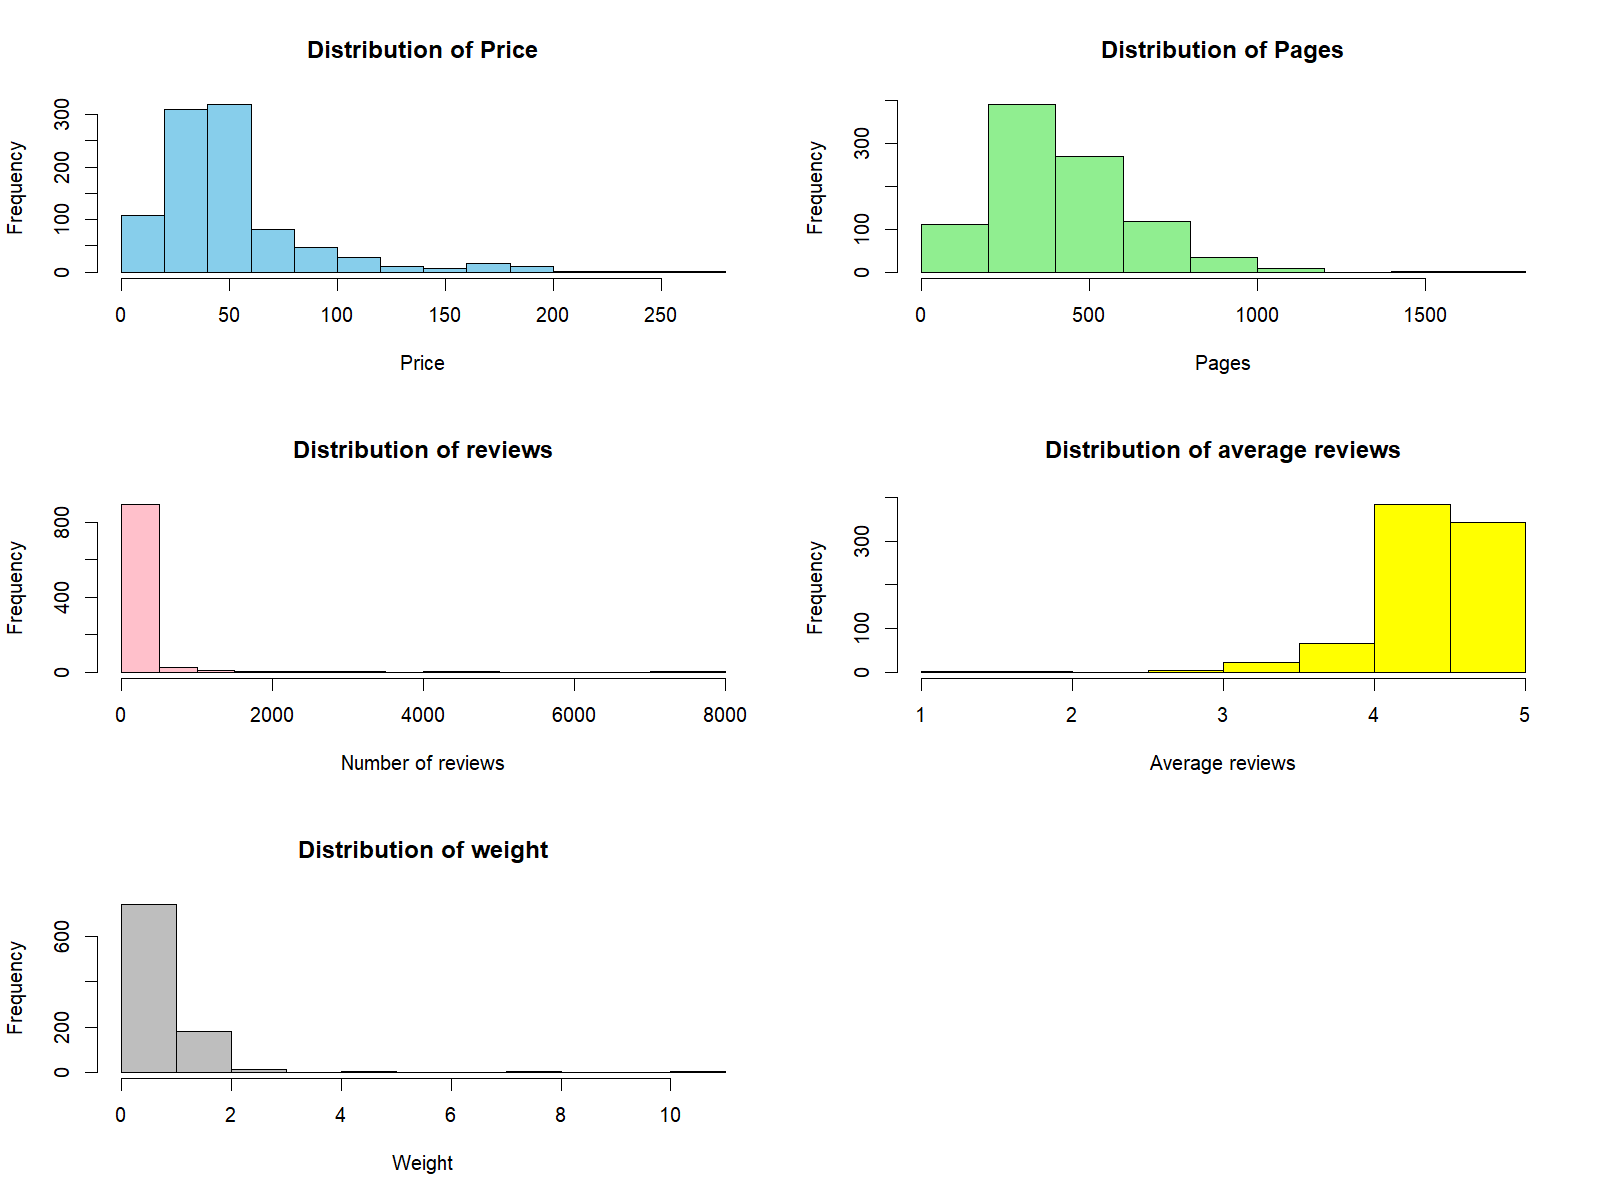
\includegraphics[width=0.95\textwidth]{plots/histograms_for_the_variability_of_data.png}
    \caption{Distributions of Price, Page Count, Review Count, Average Customer Ratings, and Book Weight}
    \label{fig:valeria_histograms}
\end{figure}
Figure~\ref{fig:valeria_histograms} presents the distributions of the five numerical variables. Price, page count, review count, and weight exhibit right-skewed distributions, whereas average customer ratings are concentrated near the upper end of the rating scale.

To see how transformation influenced the data we will plot all the numerical variables against average reviews and then their log transformed versions. Average reviews were chosen as a possible variable for prediction in the future.

\begin{figure}[H]
    \centering
    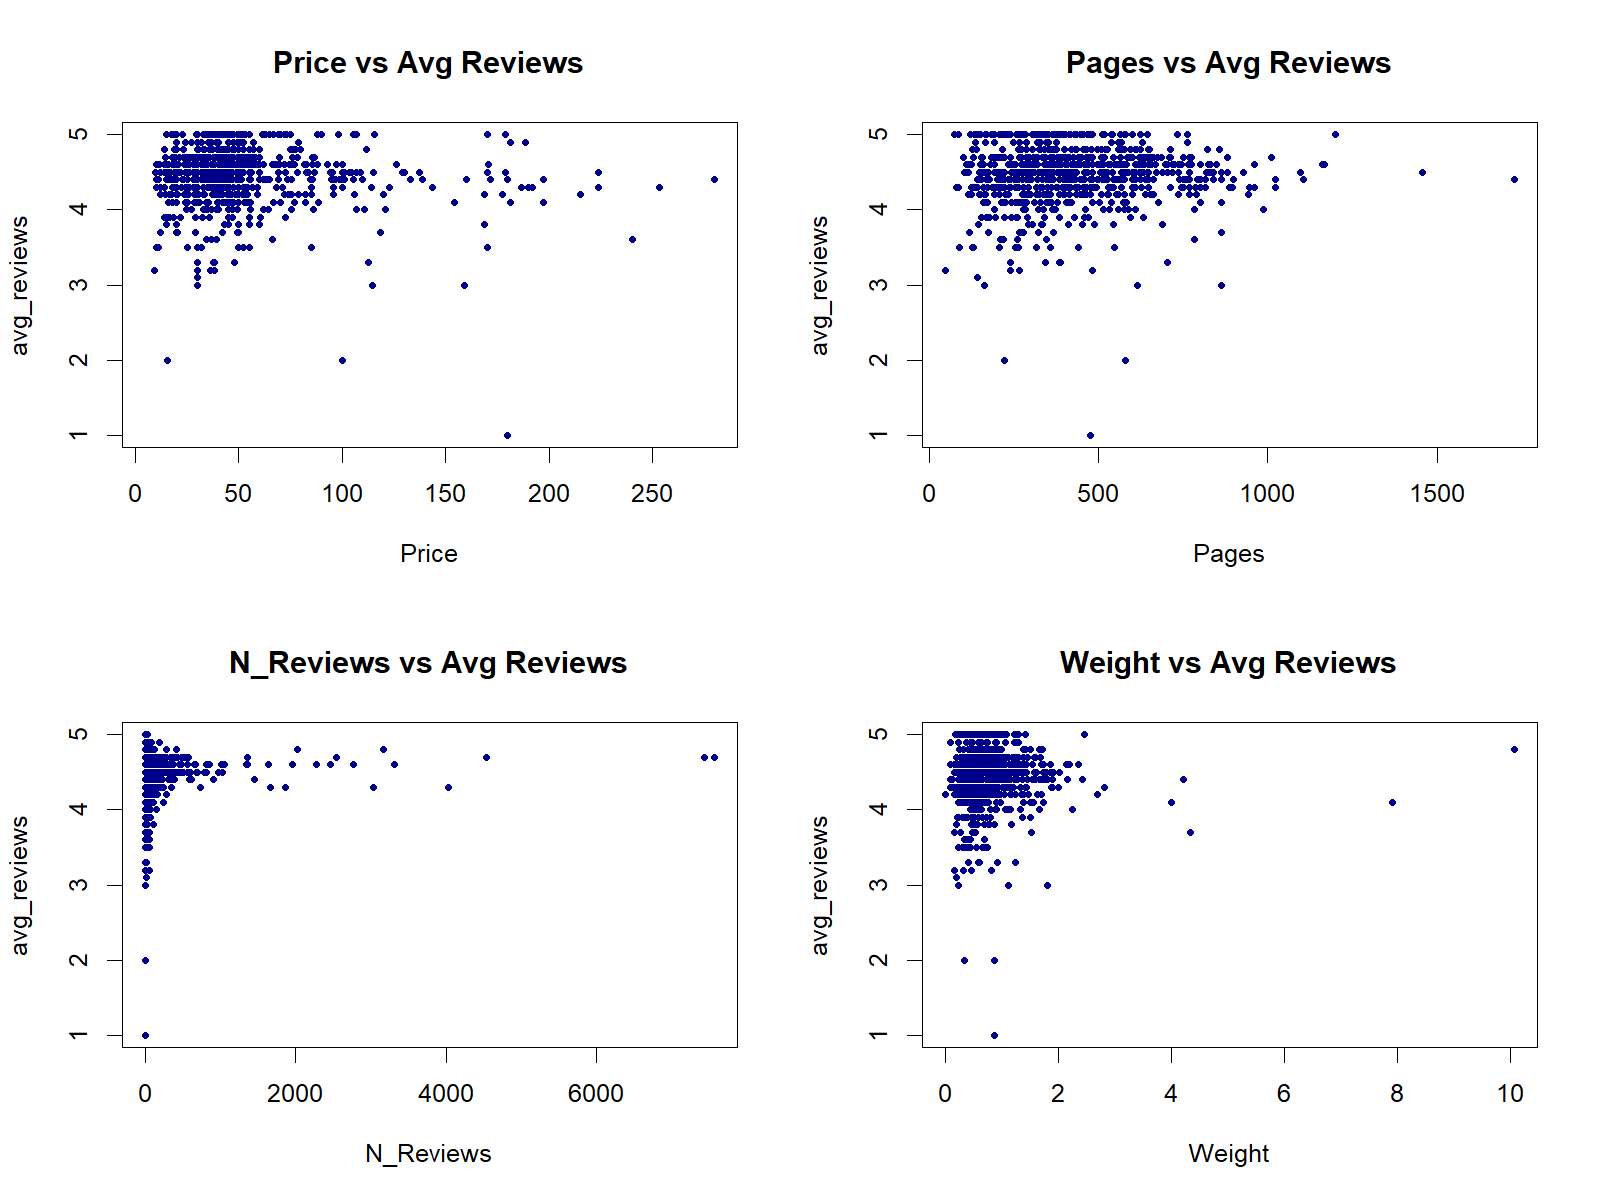
\includegraphics[width=0.85\textwidth]{plots/scatterplots_original.png}
    \caption{Original Numerical Variables versus Average Customer Ratings}
    \label{fig:original_scatterplots}
\end{figure}
\begin{figure}[H]
    \centering
    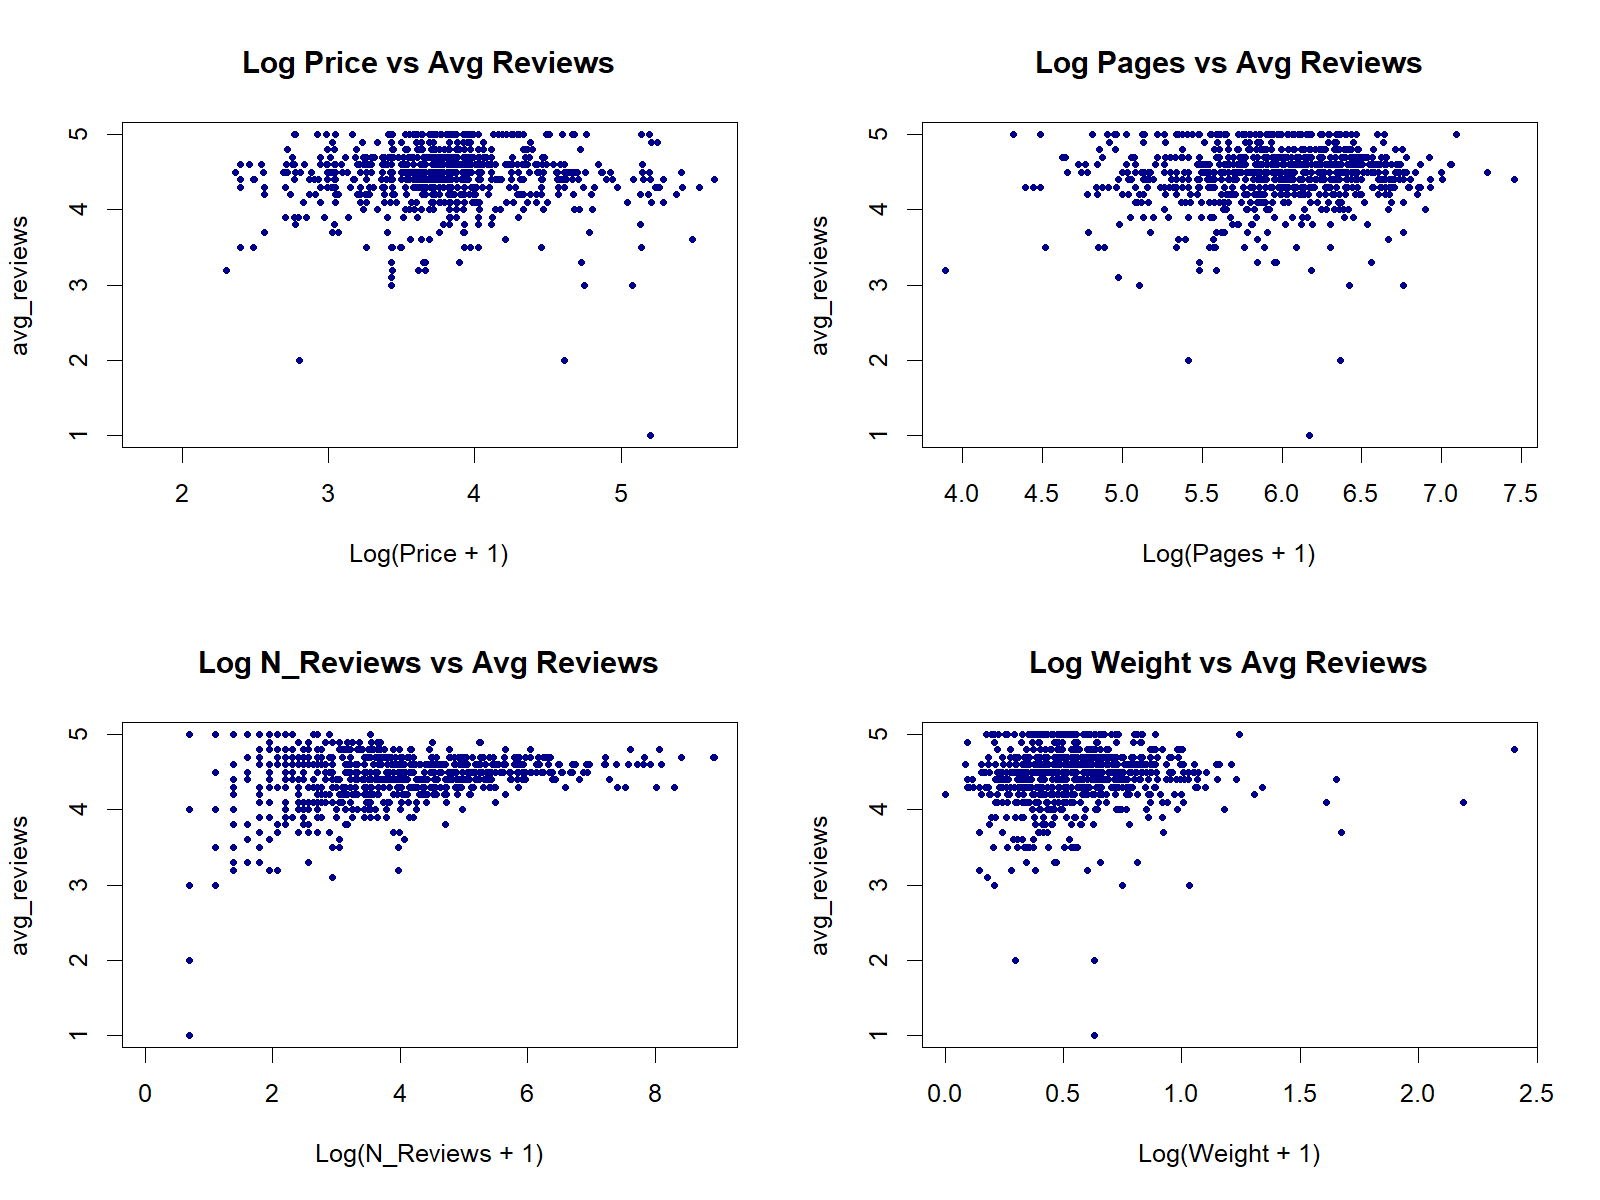
\includegraphics[width=0.85\textwidth]{plots/scatterplots_log_transformed.png}
    \caption{Log-Transformed Numerical Variables versus Average Customer Ratings}
    \label{fig:log_scatterplots}
\end{figure}

\begin{samepage}
The log-transformed variables show a more balanced
spread of observations, making their relationships
with average customer ratings easier to examine.
\end{samepage}

\newpage
\subsection{Star Rating Distribution}
To further investigate customer evaluations, the average
proportion of each category of star-ratings was calculated
among the books with available customer reviews.
Figure~\ref{fig:starratings} presents the average
distribution of ratings from one to five stars.
\begin{figure}[H]
    \centering
    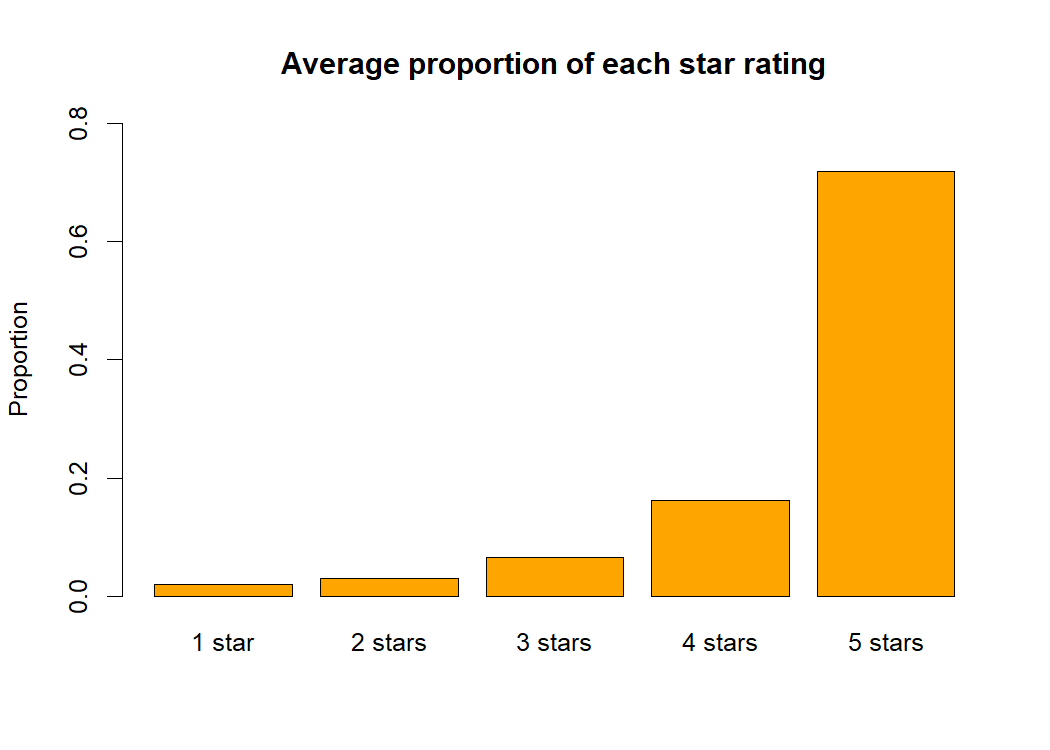
\includegraphics[width=0.85\textwidth]{plots/4_4_star_ratings.png}
    \caption{Average Distribution of Customer Star Ratings}
    \label{fig:starratings}
\end{figure}

Five-star ratings account for approximately 71.9\%
of the average rating distribution, followed by
four-star ratings at 16.2\%. Three-star ratings
represent approximately 6.7\%, while two-star and
one-star ratings account for 3.1\% and 2.2\%,
respectively.

These findings indicate that customer evaluations
are predominantly positive, consistent with the
high average ratings observed in descriptive 
statistics.

The percentages represent the mean rating proportions
across books with customer reviews, with each book contributing
equally, rather than the pooled distribution of
individual customer reviews.

\subsubsection*{Variability in Star Rating Proportions}
While Figure~\ref{fig:starratings} summarizes the
average proportion of each star-rating category,
boxplots provide additional information about
the variability of these proportions across books.

\begin{figure}[H]
    \centering
    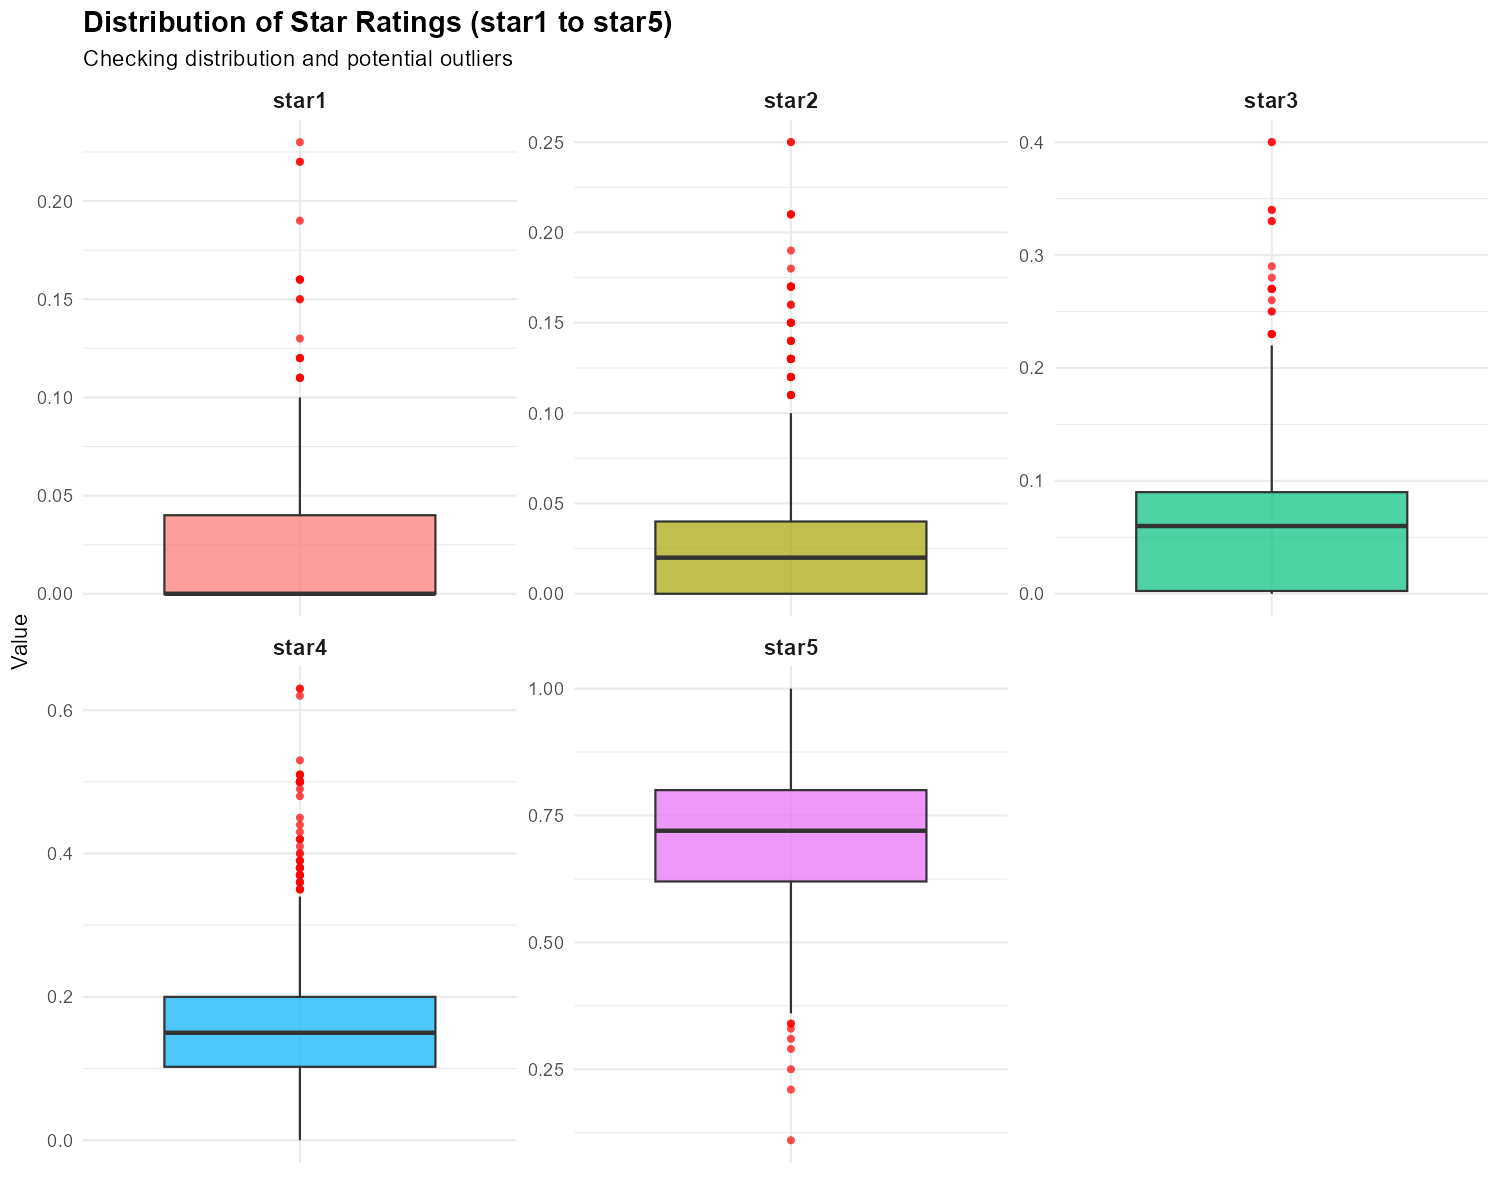
\includegraphics[width=0.95\textwidth]{plots/star_variables_boxplots.png}
    \caption{Distribution of Star Rating Proportions Across Books}
    \label{fig:starboxplots}
\end{figure}

The boxplots show that five-star ratings generally
account for the largest proportion of reviews per book,
with a median of approximately 0.72.

In contrast, one-star and two-star rating proportions
are typically close to zero, while three-star and
four-star proportions show greater variation.

Several observations appear beyond the boxplot whiskers.
However, these values are not necessarily data errors,
as unusually high or low rating proportions may reflect
genuine customer evaluations.

Together, the bar chart and boxplots provide
complementary information about the central tendency
and variability of customer rating proportions.


\subsubsection*{Distribution of Star Rating Proportions}
To further examine the distribution of customer
evaluations, histograms with density curves were
used to visualize the proportions of one-star
through five-star ratings across books.

\begin{figure}[H]
    \centering
    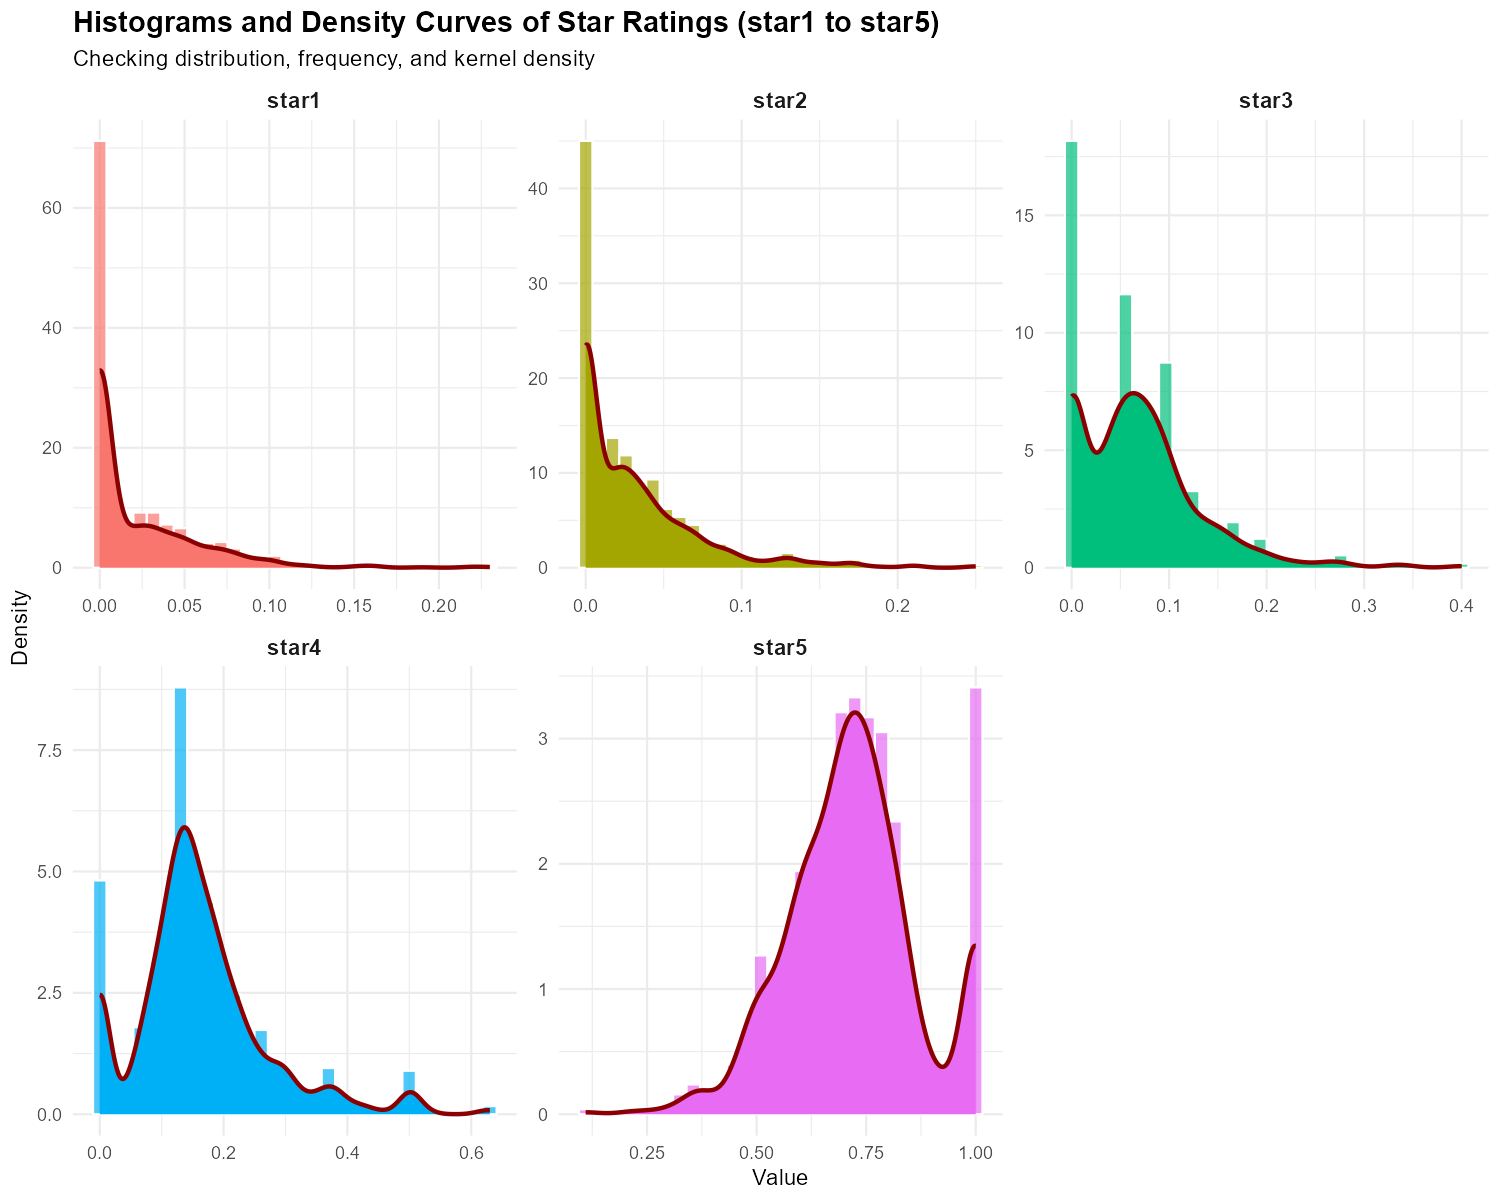
\includegraphics[width=0.95\textwidth]
    {plots/star_variables_histograms_density.png}
    \caption{Histograms and Density Curves of
    Star Rating Proportions}
    \label{fig:starhistograms}
\end{figure}

Figure~\ref{fig:starhistograms} shows that the
proportion of five-star ratings is generally
concentrated at relatively high values, with
many books having proportions between
approximately 0.60 and 0.85.

An additional concentration appears near 1.0,
indicating that some books have almost
exclusively five-star reviews.

In contrast, the distributions of one-star,
two-star, and three-star rating proportions
are strongly right-skewed, with many
observations concentrated near zero.

Four-star rating proportions generally
occupy an intermediate range, with
considerable variation across books.

These patterns are consistent with the
predominance of positive customer ratings
observed in the previous visualizations.

Because the five star-rating proportions
sum to approximately one for each reviewed
book, their distributions should not be
interpreted as independent.

\newpage
\subsection{Scatterplots and Relationships}

Scatterplots were used to visually examine relationships
between numerical variables.
Figure~\ref{fig:pagesprice} illustrates the relationship
between the number of pages and book price.
\begin{figure}[H]
    \centering
    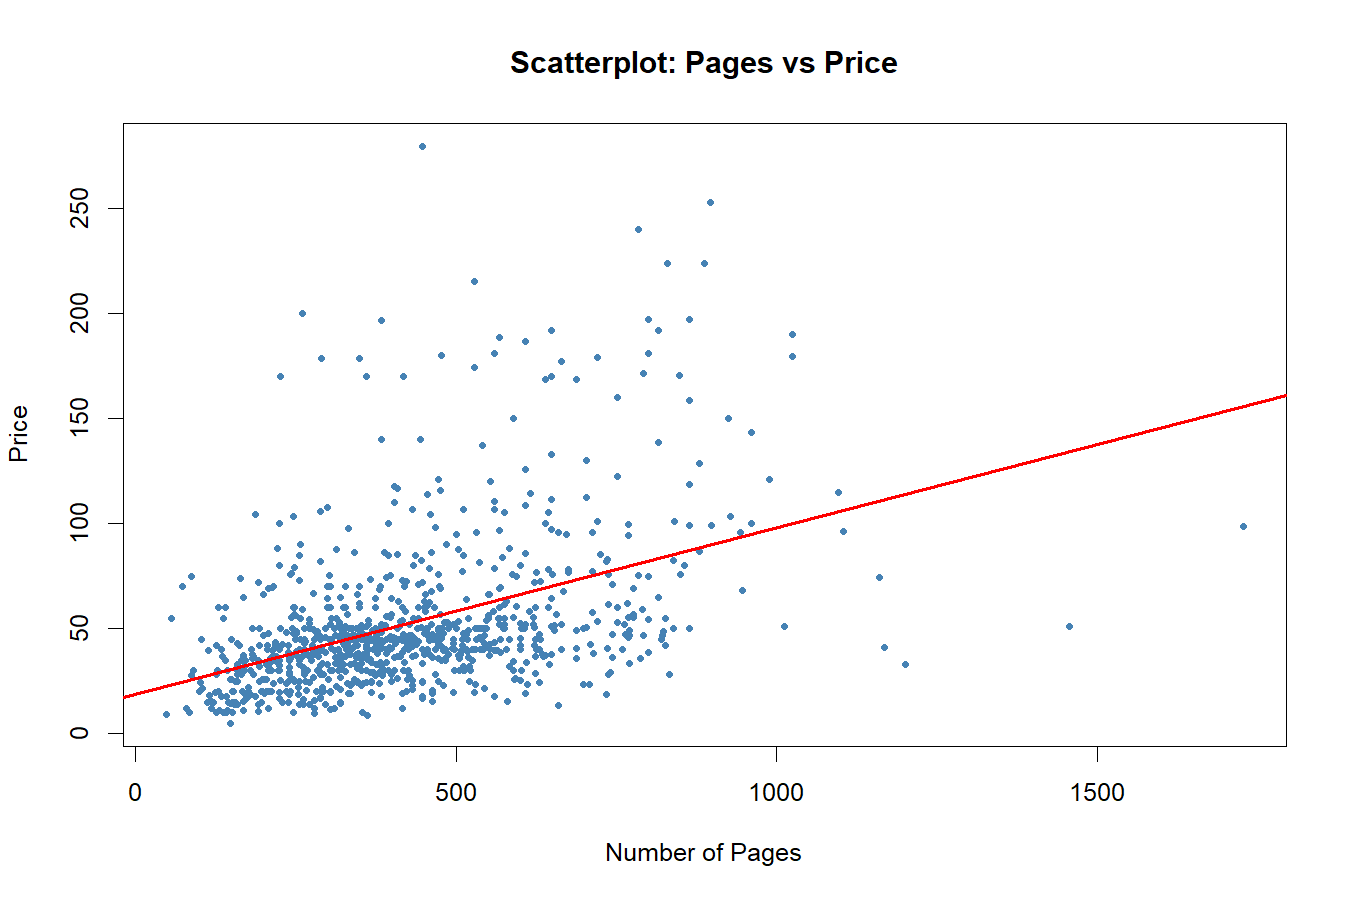
\includegraphics[width=0.85\textwidth]{plots/4_5_pages_vs_price.png}
    \caption{Relationship Between Page Count and Book Price}
    \label{fig:pagesprice}
\end{figure}

The scatterplot indicates a moderate positive relationship
between page count and price, with a Pearson correlation
coefficient of approximately 0.444.

This suggests that books with more pages tend to be more
expensive. However, considerable variation in price remains
among books with similar page counts.

The observed association does not imply that increasing
the number of pages directly causes a higher price.

The relationship between page count and book weight
was examined separately in Section~\ref{sec:cleaning},
where the effect of potentially suspicious weight
measurements was also investigated.
\subsection{Customer Reviews and Ratings}

A scatterplot was also used to examine the relationship
between average customer ratings and the number of reviews.

Since review counts are highly right-skewed, the
log-transformed number of reviews was used to improve
the visualization.

Figure~\ref{fig:reviewsrating} illustrates the relationship
between average rating and log-transformed review counts.

\begin{figure}[H]
    \centering
    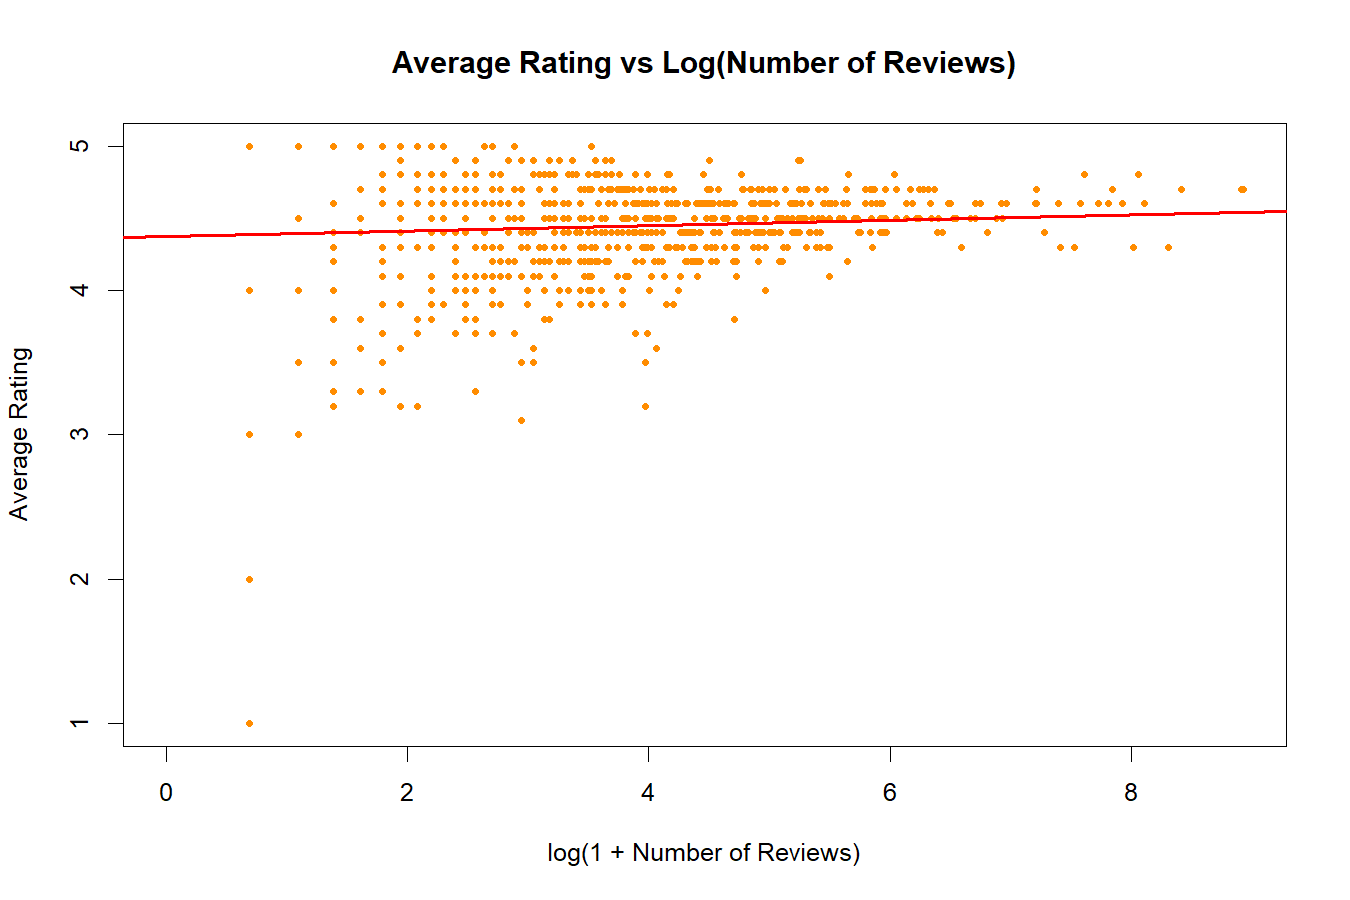
\includegraphics[width=0.85\textwidth]{plots/4_7_reviews_vs_rating.png}
    \caption{Relationship Between Average Rating and
    Log-Transformed Review Counts}
    \label{fig:reviewsrating}
\end{figure}

The Pearson correlation coefficient between average rating
and log-transformed review counts was approximately 0.074,
indicating a very weak positive linear relationship.

The scatterplot suggests that books receiving more reviews
do not necessarily have higher average ratings. Books with
similar review counts may have substantially different
ratings.

Overall, the number of reviews appears to have little
linear association with the average customer rating
in this dataset.

\newpage
\subsection{Correlation Matrix Heatmap}
To analyse the correlations between the main numerical
variables, a Pearson correlation matrix was constructed
using price, pages, number of reviews, average customer
ratings, and book weight.
\begin{figure}[H]
    \centering
    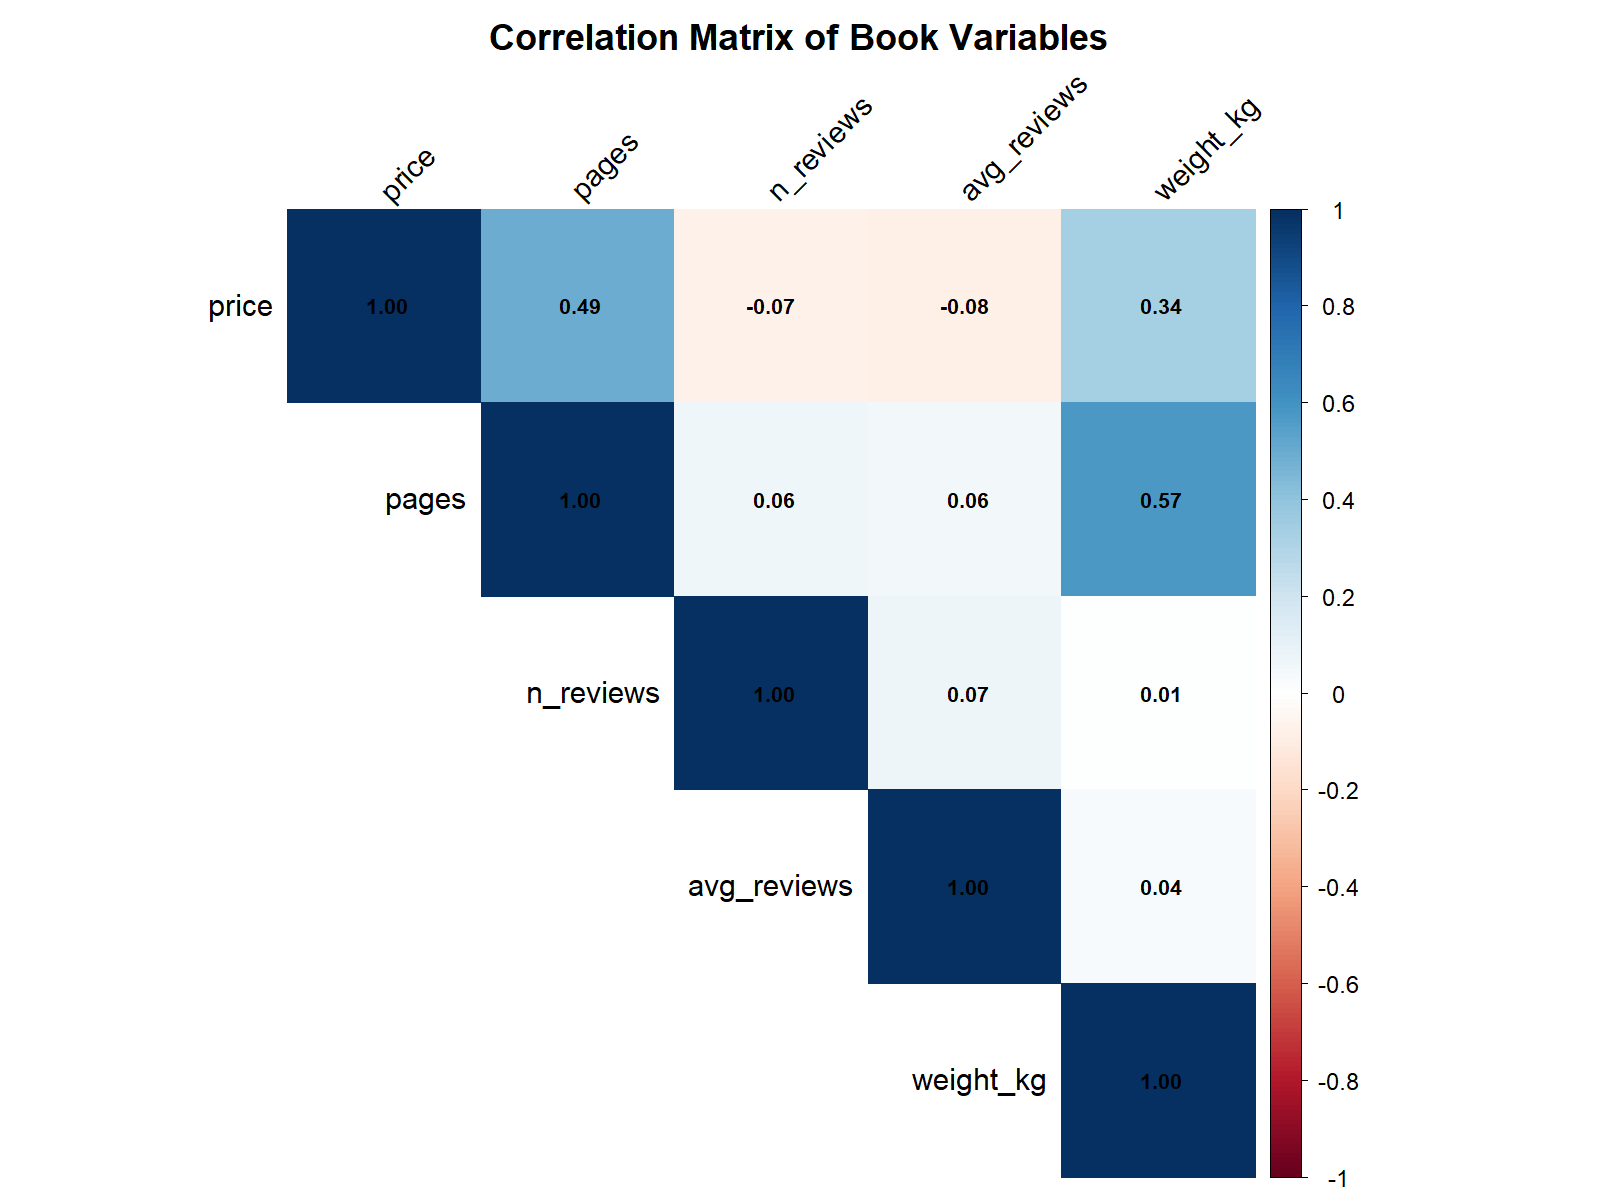
\includegraphics[width=0.85\textwidth]{plots/correlation_matrix_basic.png}
    \caption{Correlation Matrix of Price, Pages, Review Counts, Average Ratings, and Weight}
    \label{fig:correlation_basic}
\end{figure}
According to Figure~\ref{fig:correlation_basic}, price and number of pages have a moderate positive correlation ($r = 0.49$). This may be explained by the fact that larger books require more physical materials.

A positive correlation is also observed between price and weight ($r = 0.34$), while pages and weight show a stronger positive correlation ($r = 0.57$).

However, average customer ratings show correlations
close to zero with price, pages, number of reviews,
and weight. These results suggest that the selected
book characteristics have very weak linear associations
with average customer ratings.

To extend this analysis, the following correlation
matrix includes the individual star-rating proportions.
\begin{figure}[H]
    \centering
    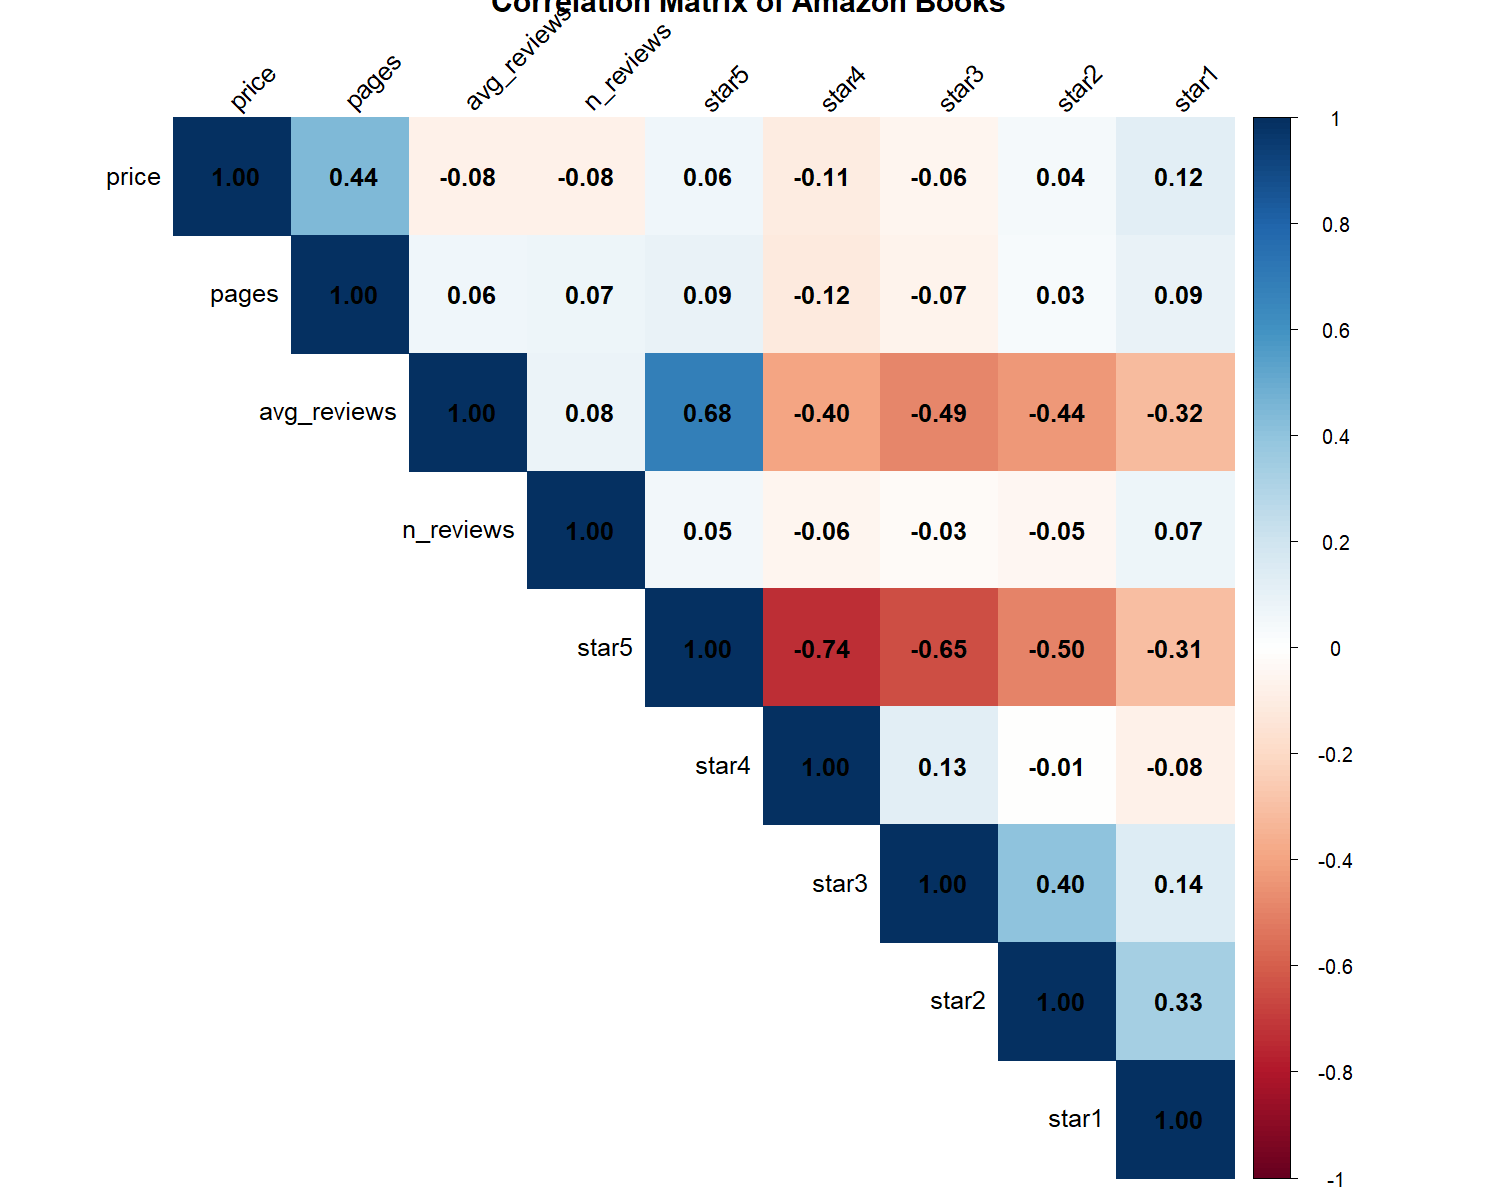
\includegraphics[width=0.95\textwidth]{plots/correlation_matrix_heatmap.png}
    \caption{Pearson Correlation Matrix of Numerical Variables}
    \label{fig:correlationheatmap}
\end{figure}
Figure~\ref{fig:correlationheatmap} shows a moderate positive correlation between book price and page count ($r \approx 0.44$), consistent with the corresponding scatterplot.

Average customer ratings show a strong positive correlation with the proportion of five-star reviews ($r \approx 0.68$). Conversely, the proportion of five-star reviews is negatively
correlated with four-star ($r \approx -0.74$) and three-star ($r \approx -0.65$) review proportions.

These relationships should be interpreted carefully because
the star-rating proportions sum to one and the average rating
is mathematically related to their distribution.

In contrast, the number of customer reviews exhibits very
weak linear correlations with both average ratings
($r \approx 0.08$) and book prices ($r \approx -0.08$).

Overall, the heatmap provides a broader view of the linear
relationships within the dataset, complementing the more
detailed scatterplot analysis.


\subsection{Pairwise Scatter Plot Matrix}
A pairwise scatter plot matrix was used to explore
relationships among the main numerical variables,
including price, page count, average customer rating,
review count, and star-rating proportions.
\begin{figure}[H]
    \centering
    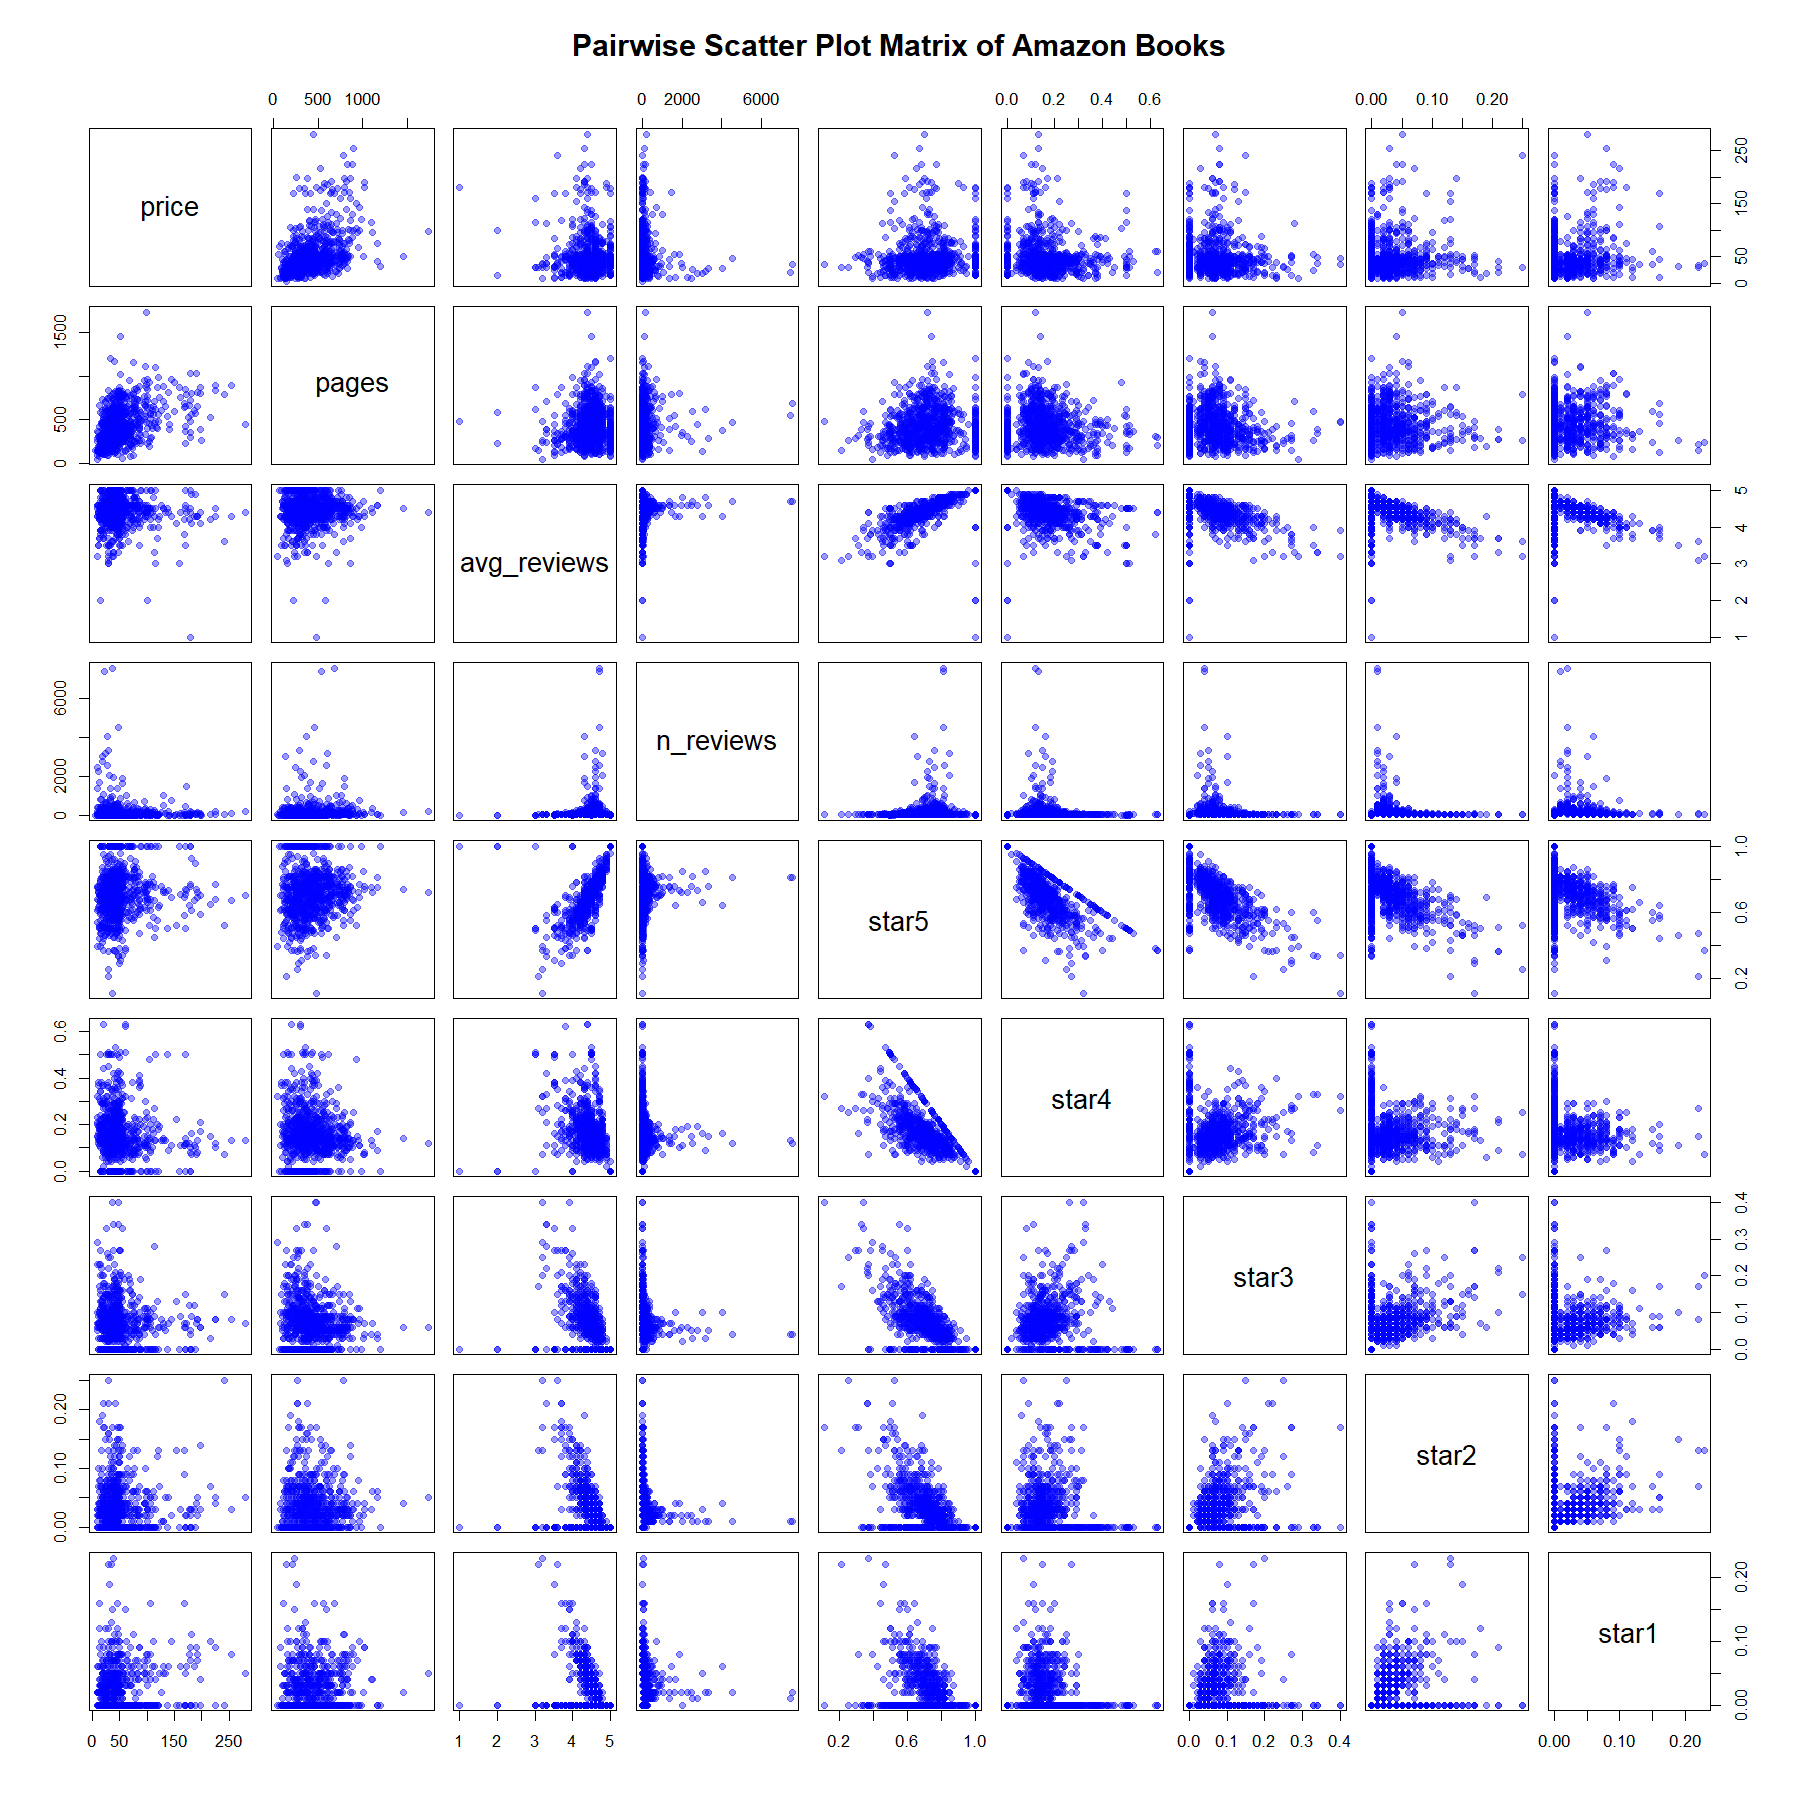
\includegraphics[width=0.95\textwidth]
    {plots/pairwise_scatterplot_matrix.png}
    \caption{Pairwise Scatter Plot Matrix of Amazon Books}
    \label{fig:pairs_plot}
\end{figure}
The scatter plot matrix provides a broader overview
of the relationships between numerical variables. The plots involving review counts reveal a strong
concentration of observations at relatively low
values, together with a small number of books
receiving exceptionally high numbers of reviews. The relationship between price and page count
shows a moderate positive association, consistent
with the individual scatterplot analysis.
The star-rating proportions exhibit constrained
patterns because the proportions for each reviewed
book sum approximately to one.

Overall, the pairwise scatter plot matrix
complements the correlation heatmap by providing
a visual overview of the relationships, clusters,
and potential outliers in the dataset.


\subsection{Categorical Analysis}
Categorical variables were examined to investigate
the distribution of customer review availability
and book languages.

Two bar charts were used to visualize the
frequency counts of the variables
\texttt{has\_reviews} and \texttt{language\_clean}.
\begin{figure}[H]
    \centering

    \begin{subfigure}[b]{0.48\textwidth}
        \centering
        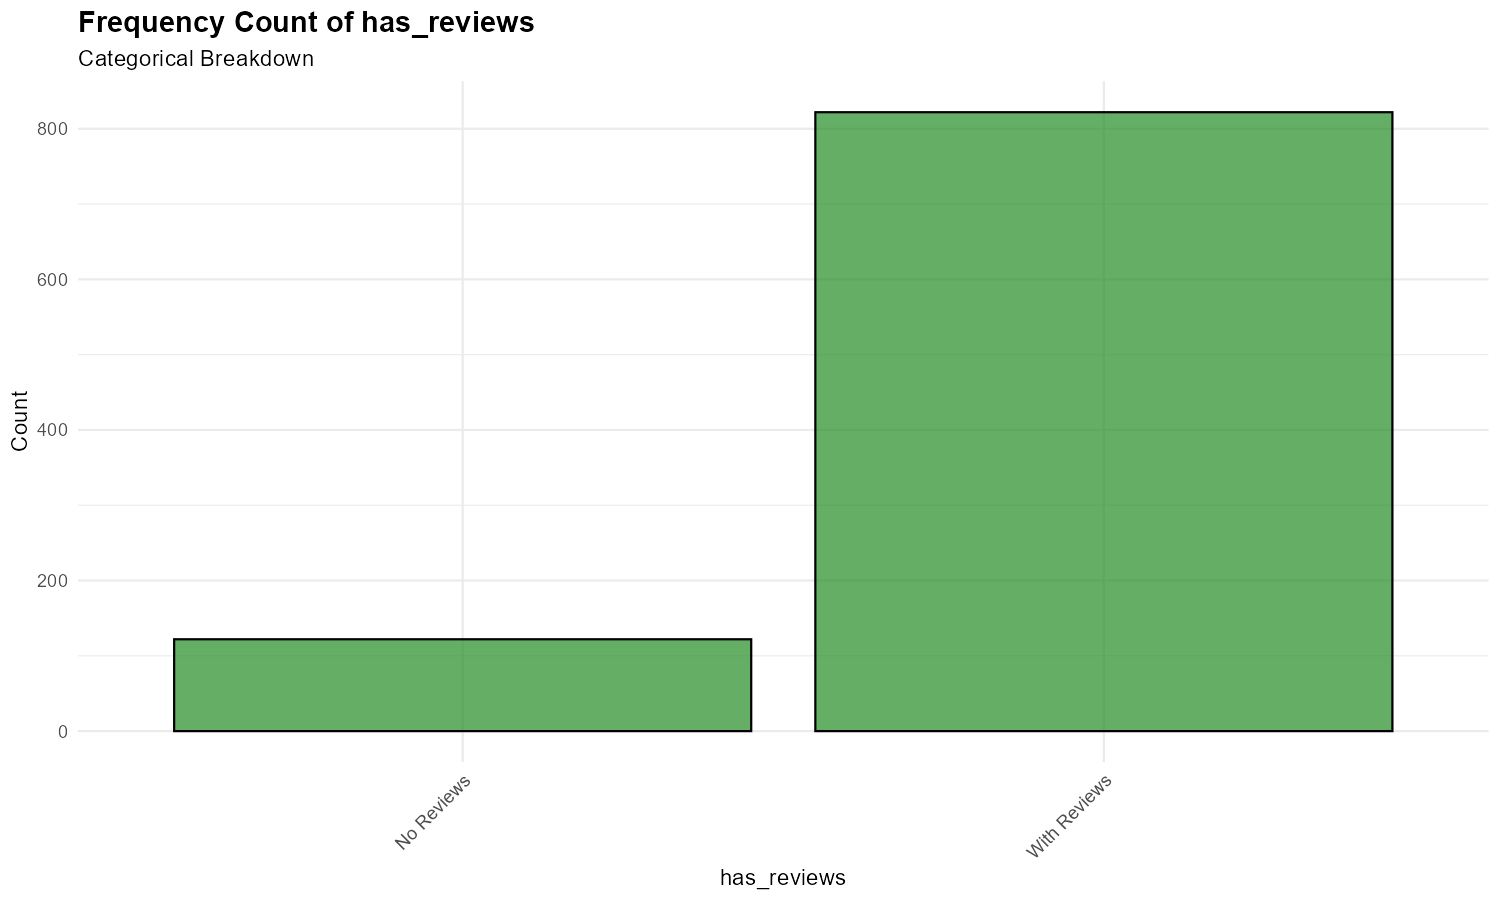
\includegraphics[width=\textwidth]
        {plots/categorical_bar_has_reviews.png}
        \caption{Availability of Customer Reviews}
        \label{fig:bar_has_reviews}
    \end{subfigure}
    \hfill
    \begin{subfigure}[b]{0.48\textwidth}
        \centering
        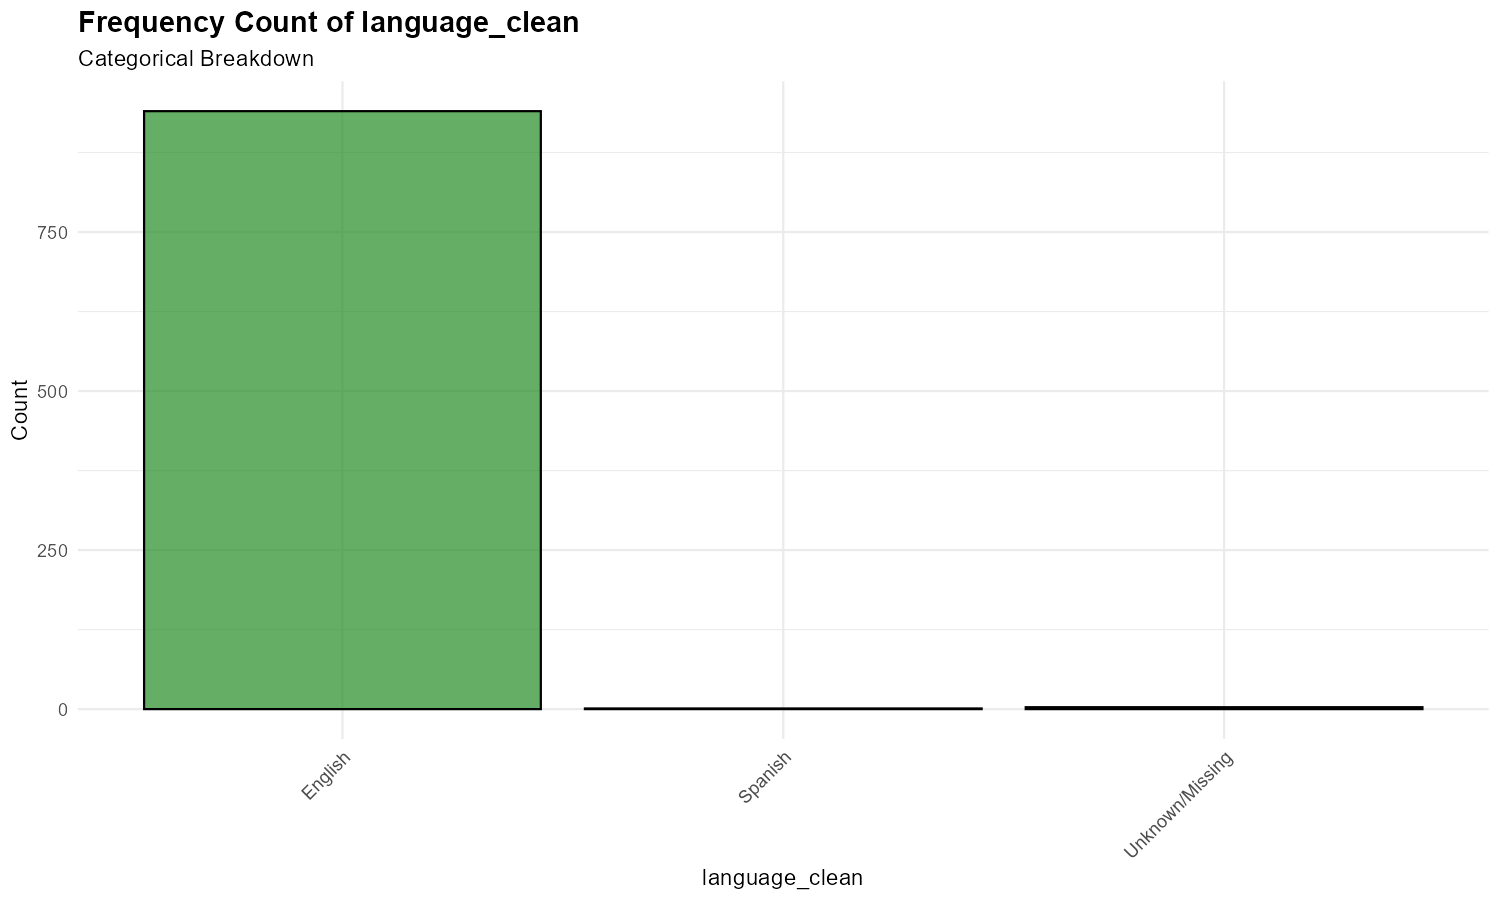
\includegraphics[width=\textwidth]
        {plots/categorical_bar_language_clean.png}
        \caption{Distribution of Book Languages}
        \label{fig:bar_language_clean}
    \end{subfigure}

    \caption{Categorical Breakdown of Review
    Availability and Book Languages}
    \label{fig:categorical_bars}
\end{figure}

\subsubsection*{Customer Review Availability}

The dataset contains 945 books, of which 822
(approximately 87.0\%) have at least one
customer review, while 123 (approximately
13.0\%) have no customer reviews.

This indicates that most books in the dataset
have received customer feedback.

However, the absence of reviews for some books
limits the availability of rating-related
information for these observations.

\subsubsection*{Distribution of Book Languages}

The distribution of book languages shows that
English is the predominant language in the
dataset, while other languages are represented
by relatively few observations.

This imbalance indicates that the dataset
primarily reflects English-language
data science books.

Consequently, comparisons between language
categories should be interpreted cautiously,
particularly when some categories contain
very few books.

Overall, the categorical analysis complements
the numerical exploration by highlighting
differences in review availability and
language representation across the dataset.

% ==========================================
% 6. HYPOTHESIS TESTING
% ==========================================

\newpage
\section{Hypothesis Testing and Empirical Findings}


To formally evaluate the underlying relationships and market dynamics prior to econometric modeling, five primary statistical hypotheses were formulated and empirically tested.

\subsection{Hypothesis 1: The Effect of Page Count on Book Price and Non-Parametric Modeling}

\begin{itemize}
    \item \textbf{Null Hypothesis ($H_0$):} There is no correlation between the number of pages (\texttt{pages}) and the log-transformed book price ($\beta = 0$).

    \item \textbf{Alternative Hypothesis ($H_1$):} Book page count is significantly correlated with price ($\beta \neq 0$).
\end{itemize}

\begin{figure}[H]
    \centering
    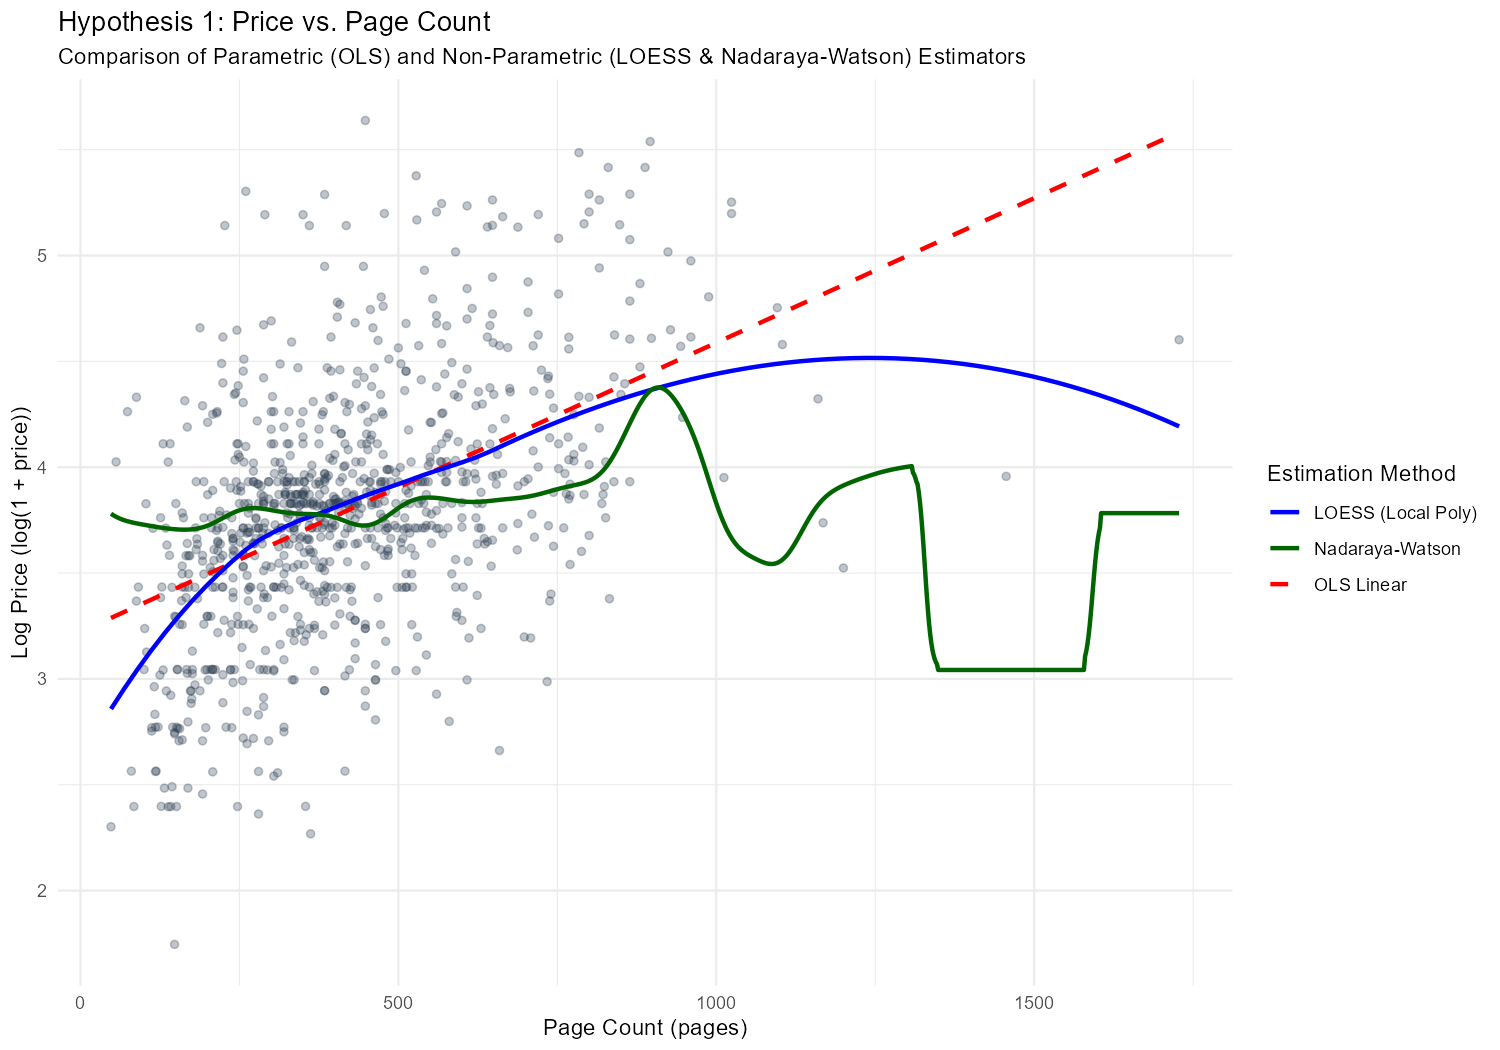
\includegraphics[width=0.85\textwidth]{plots/hypothesis_1_price_pages.png}
    \caption{Hypothesis 1: Comparison of Parametric (OLS) and Non-Parametric Estimators}
    \label{fig:h1_plot}
\end{figure}
\subsubsection*{Empirical Results and Statistical Testing}
The Pearson product-moment correlation test revealed a statistically significant positive relationship between page count and $\log(1 + \text{price})$, yielding a correlation coefficient of $r = 0.4862$ ($t = 16.95, df = 928, p < 2.2 \times 10^{-16}$) with a 95\% confidence interval ranging from $0.4355$ to $0.5338$. To accommodate zero values, the transformation \(\log(1+x)\) can be used where appropriate.

\subsubsection*{Graph Interpretation and Non-Parametric Benchmarking}
Evaluating the comparative estimator graph (OLS linear vs. LOESS vs. Nadaraya--Watson) reveals distinct structural behaviors across the distribution:
\begin{itemize}
    \item In the primary density region (from 0 to approximately 800 pages), the parametric OLS trend line and the non-parametric LOESS curve closely align, corroborating a stable positive association between physical volume and retail pricing.

    \item In the right-tail boundary region (exceeding 1,000 pages), the Nadaraya--Watson kernel regression exhibits severe boundary bias and local fluctuations due to data sparsity.

    \item Conversely, the LOESS (local polynomial regression) estimator provides a robust, smooth trajectory that successfully handles boundary effects without imposing strict global linearity, while the linear OLS tends to extrapolate upward in the sparse tail.
\end{itemize}

\paragraph{Methodological Conclusion:} The empirical evidence confirms that physical volume (scaling of material and production costs) exerts a tangible upward pressure on retail pricing, validating pages as a core structural predictor while robustly controlling for non-linearities and boundary constraints.


\subsection{Hypothesis 2: Price Differentiation Based on Review Engagement}

\begin{itemize}
    \item \textbf{Null Hypothesis ($H_0$):} The mean log-price of books without reviews (\texttt{No Reviews}) is equal to the mean log-price of books with active reviews (\texttt{With Reviews}).

    \item \textbf{Alternative Hypothesis ($H_1$):} There is a statistically significant difference in mean pricing between reviewed and unreviewed titles.
\end{itemize}

\begin{figure}[htbp]
    \centering
    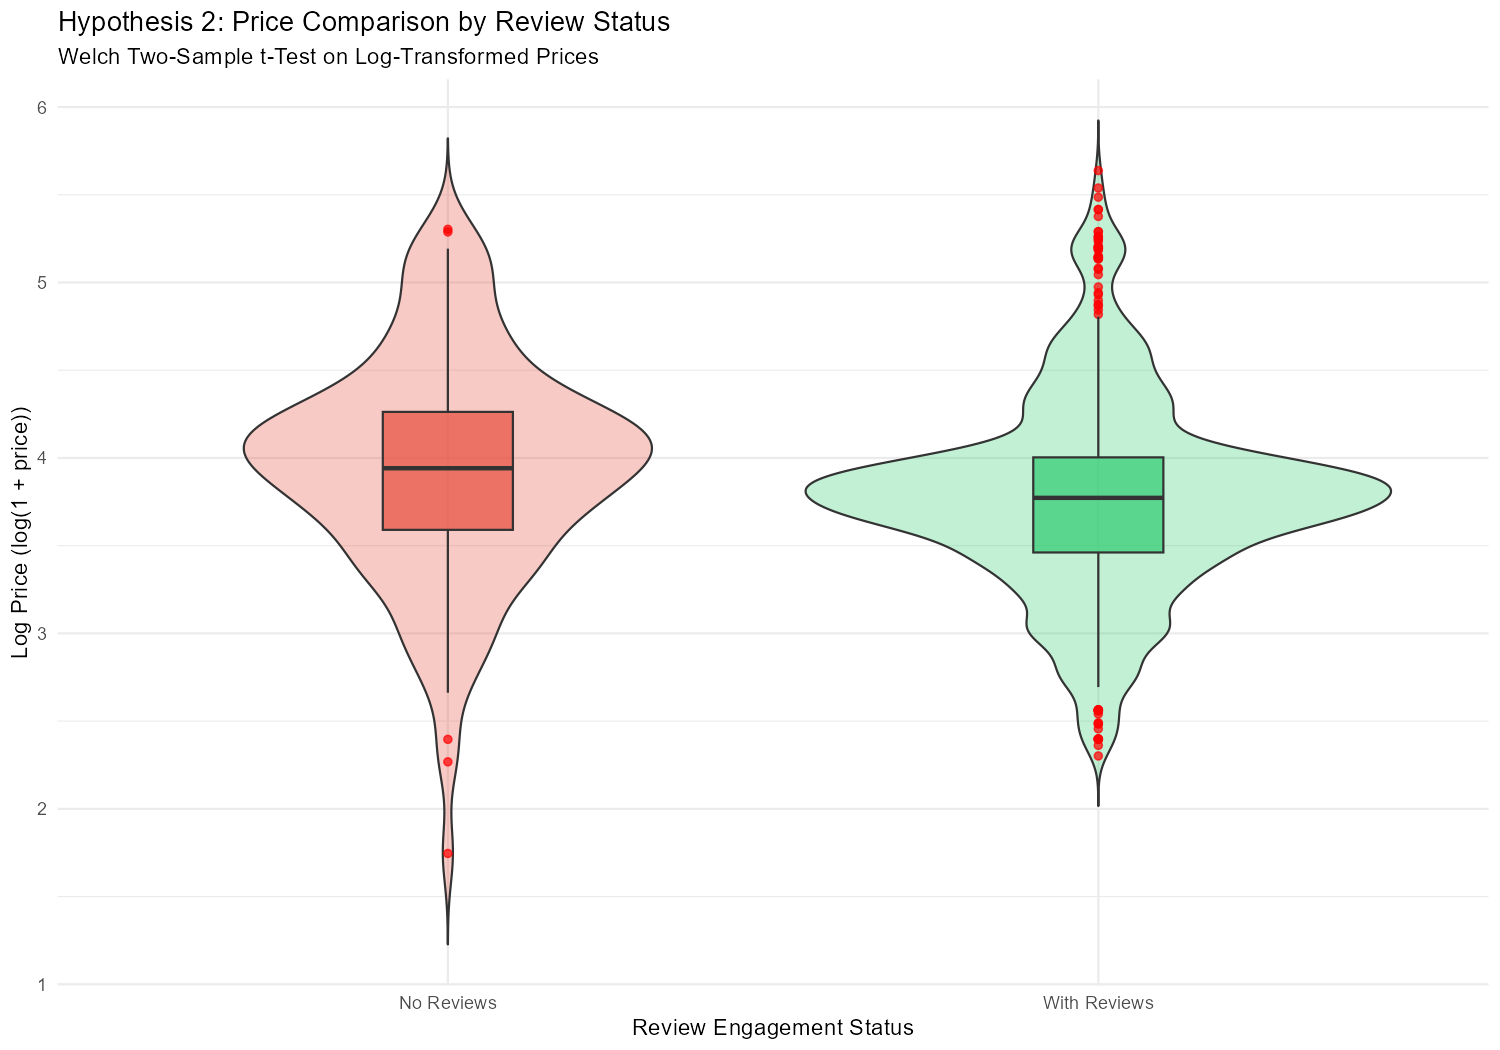
\includegraphics[width=0.85\textwidth]{plots/hypothesis_2_price_reviews.png}
    \caption{Hypothesis 2: Price Comparison by Review Engagement Status}
    \label{fig:h2_plot}
\end{figure}

\subsubsection*{Empirical Results and Group Estimates}

A Welch two-sample t-test was conducted on $\log(1 + \text{price})$ to evaluate pricing disparities while controlling for variance heterogeneity. Results demonstrate a statistically significant difference in means ($t = 2.7169, df = 149.93, p = 0.007365$). The 95\% confidence interval ranges from $0.04539$ to $0.28747$, rejecting the null hypothesis at $\alpha = 0.01$.

\begin{itemize}
    \item \textbf{No Reviews Group:} Mean $\log(1 + \text{price}) = 3.943155$.

    \item \textbf{With Reviews Group:} Mean $\log(1 + \text{price}) = 3.776725$.
\end{itemize}

\paragraph{Economic Interpretation:} Unreviewed or newly listed titles carry higher baseline list prices. This aligns with pricing lifecycle strategies in e-commerce: unreviewed products often launch at premium list prices, whereas products with high consumer engagement undergo competitive discounting or promotional adjustments over time.


\subsection{Hypothesis 3: Variance in Ratings Across Publication Languages}

\begin{itemize}
    \item \textbf{Null Hypothesis ($H_0$):} The mean average review rating (\texttt{avg\_reviews}) does not differ significantly across language categories.

    \item \textbf{Alternative Hypothesis ($H_1$):} Review ratings vary significantly across publication languages.
\end{itemize}

\begin{figure}[htbp]
    \centering
    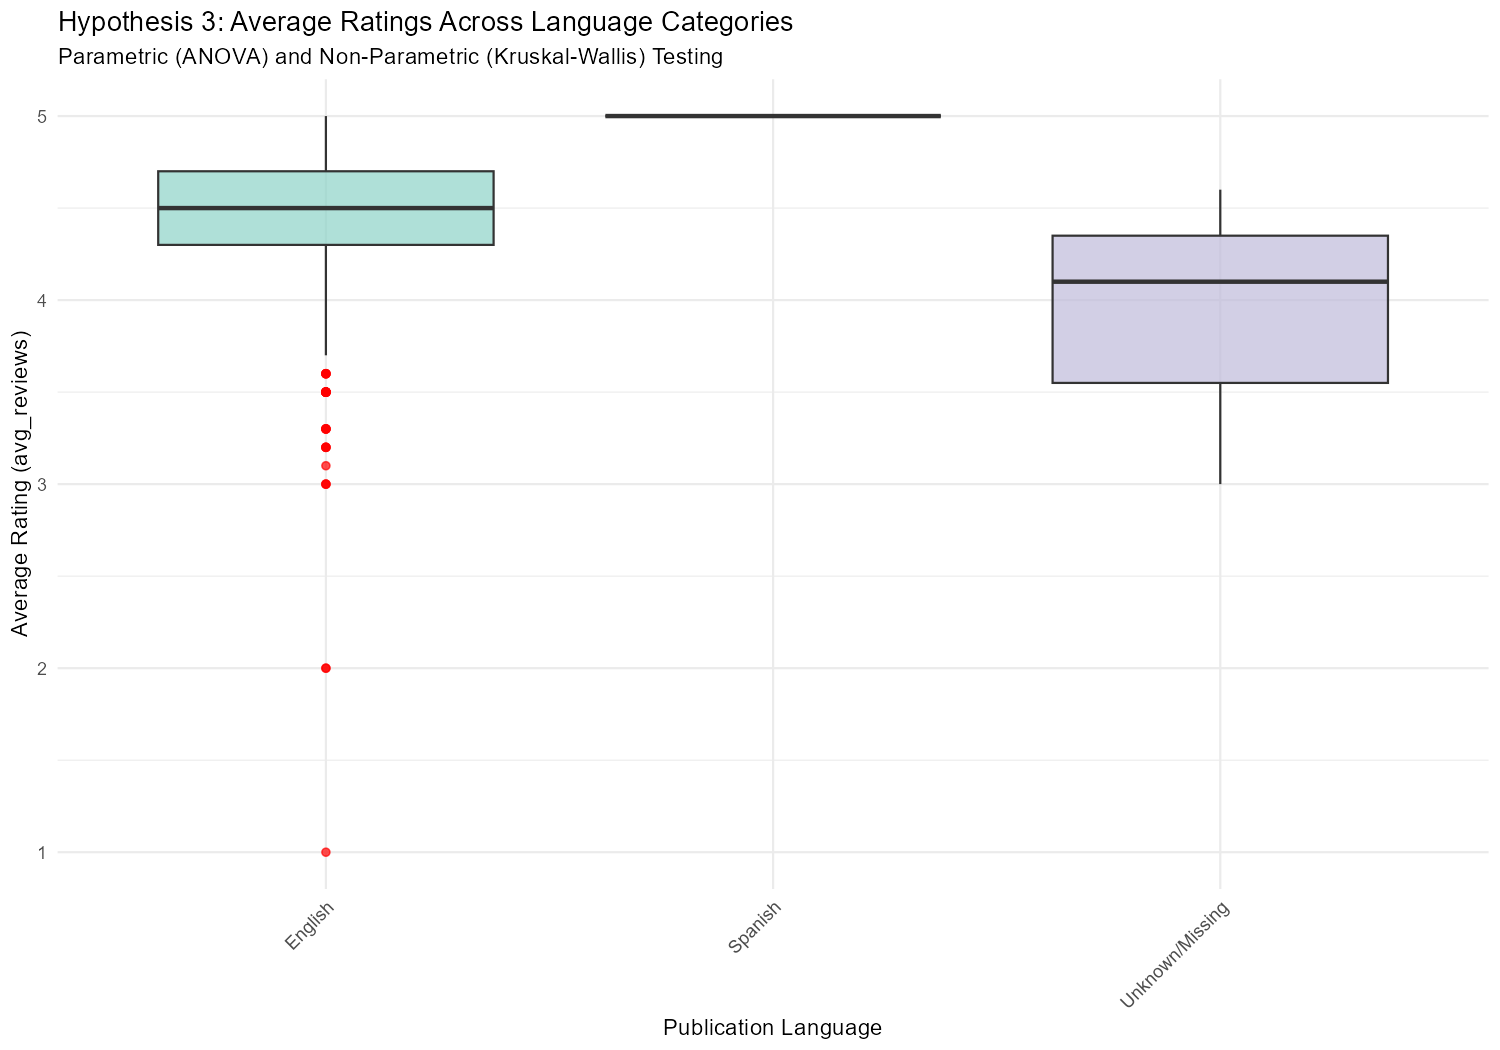
\includegraphics[width=0.85\textwidth]{plots/hypothesis_3_ratings_languages.png}
    \caption{Hypothesis 3: Average Ratings Across Language Categories}
    \label{fig:h3_plot}
\end{figure}

\subsubsection*{Empirical Results and Methodological Conclusion}

Parametric ANOVA revealed a marginally significant effect ($F = 3.734, df = 2, p = 0.0243$). However, the non-parametric Kruskal-Wallis test yielded a non-significant result ($\chi^2 = 4.4508, df = 2, p = 0.108$). Because the non-parametric test fails to reject the null hypothesis, we conclude that publication language does not exert a robust systematic effect on average ratings once distributional asymmetries are controlled for.


\subsection{Hypothesis 4: Review Volume vs. Book Pricing Dynamics}

\begin{itemize}
    \item \textbf{Null Hypothesis ($H_0$):} There is no monotonic correlation between the number of customer reviews (\texttt{n\_reviews}) and the log-transformed book price.

    \item \textbf{Alternative Hypothesis ($H_1$):} There is a statistically significant monotonic correlation between review volume and book price.
\end{itemize}

\begin{figure}[htbp]
    \centering
    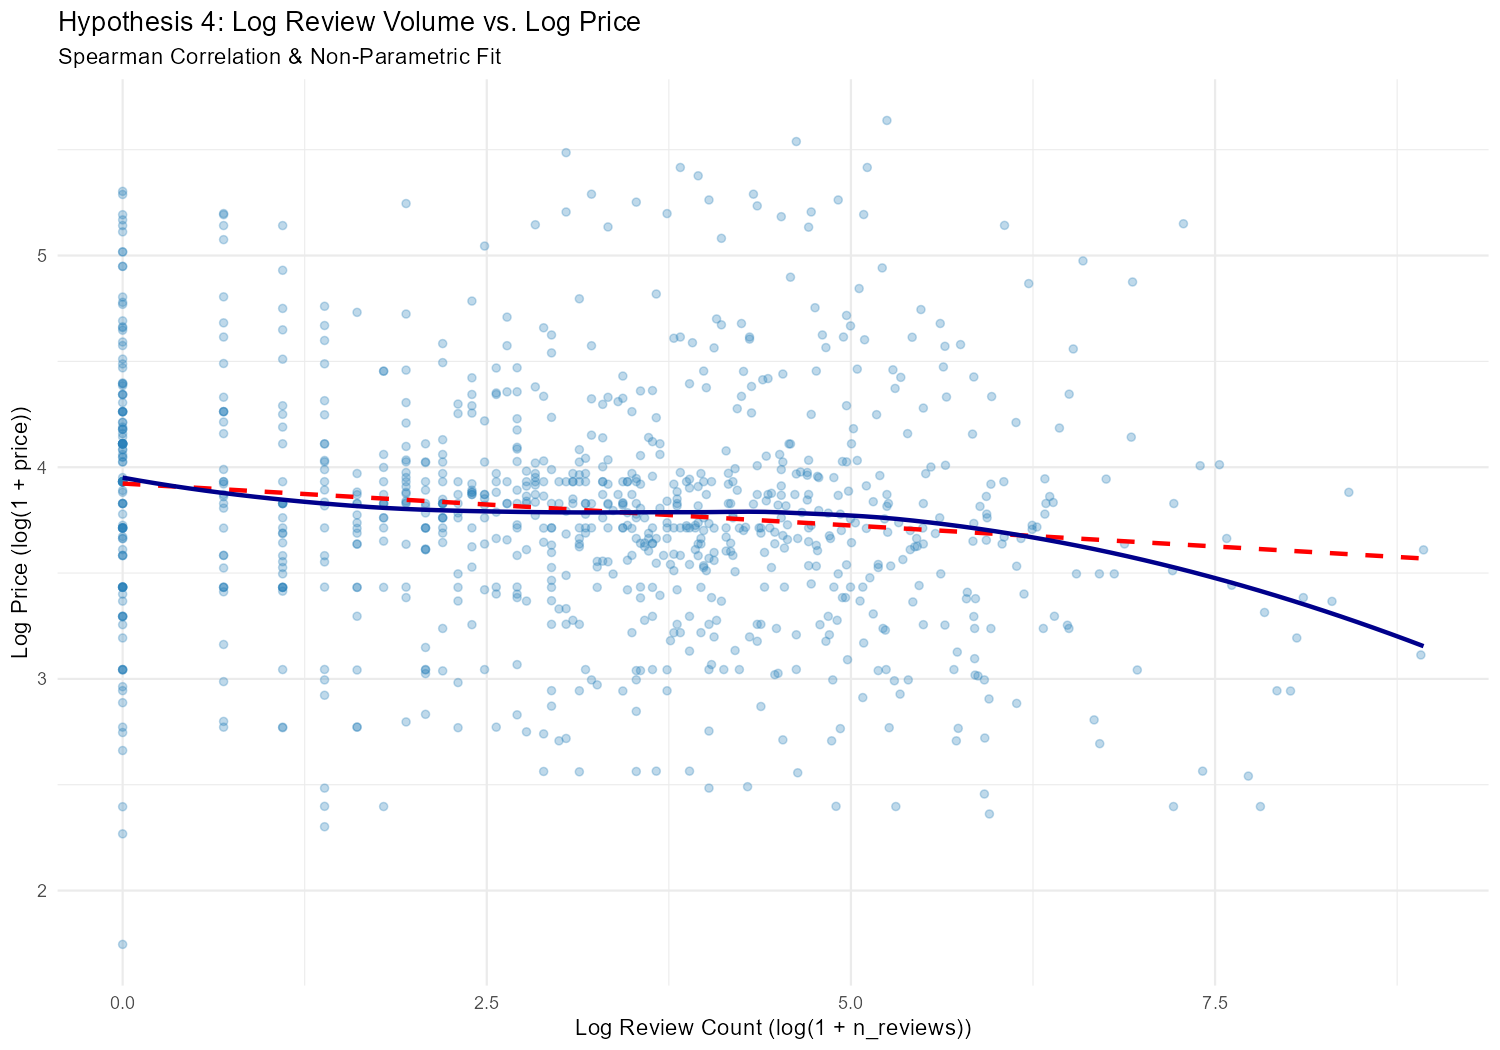
\includegraphics[width=0.85\textwidth]{plots/hypothesis_4_reviews_price.png}
    \caption{Hypothesis 4: Relationship Between Review Volume and Book Price}
    \label{fig:h4_plot}
\end{figure}

\subsubsection*{Empirical Results and Statistical Testing}

The Spearman rank correlation test revealed a statistically significant negative association between the number of customer reviews and log-transformed book price ($\rho = -0.1554$, $S = 160966486$, $p = 1.647 \times 10^{-6}$).

The null hypothesis is rejected, indicating a weak but statistically significant negative monotonic relationship between review volume and book price.


\subsection{Hypothesis 5: Average Customer Rating vs. Book Price}

\begin{itemize}
    \item \textbf{Null Hypothesis ($H_0$):} There is no monotonic correlation between the average customer rating (\texttt{avg\_reviews}) and the log-transformed book price.

    \item \textbf{Alternative Hypothesis ($H_1$):} There is a statistically significant monotonic correlation between average customer ratings and book price.
\end{itemize}

\begin{figure}[htbp]
    \centering
    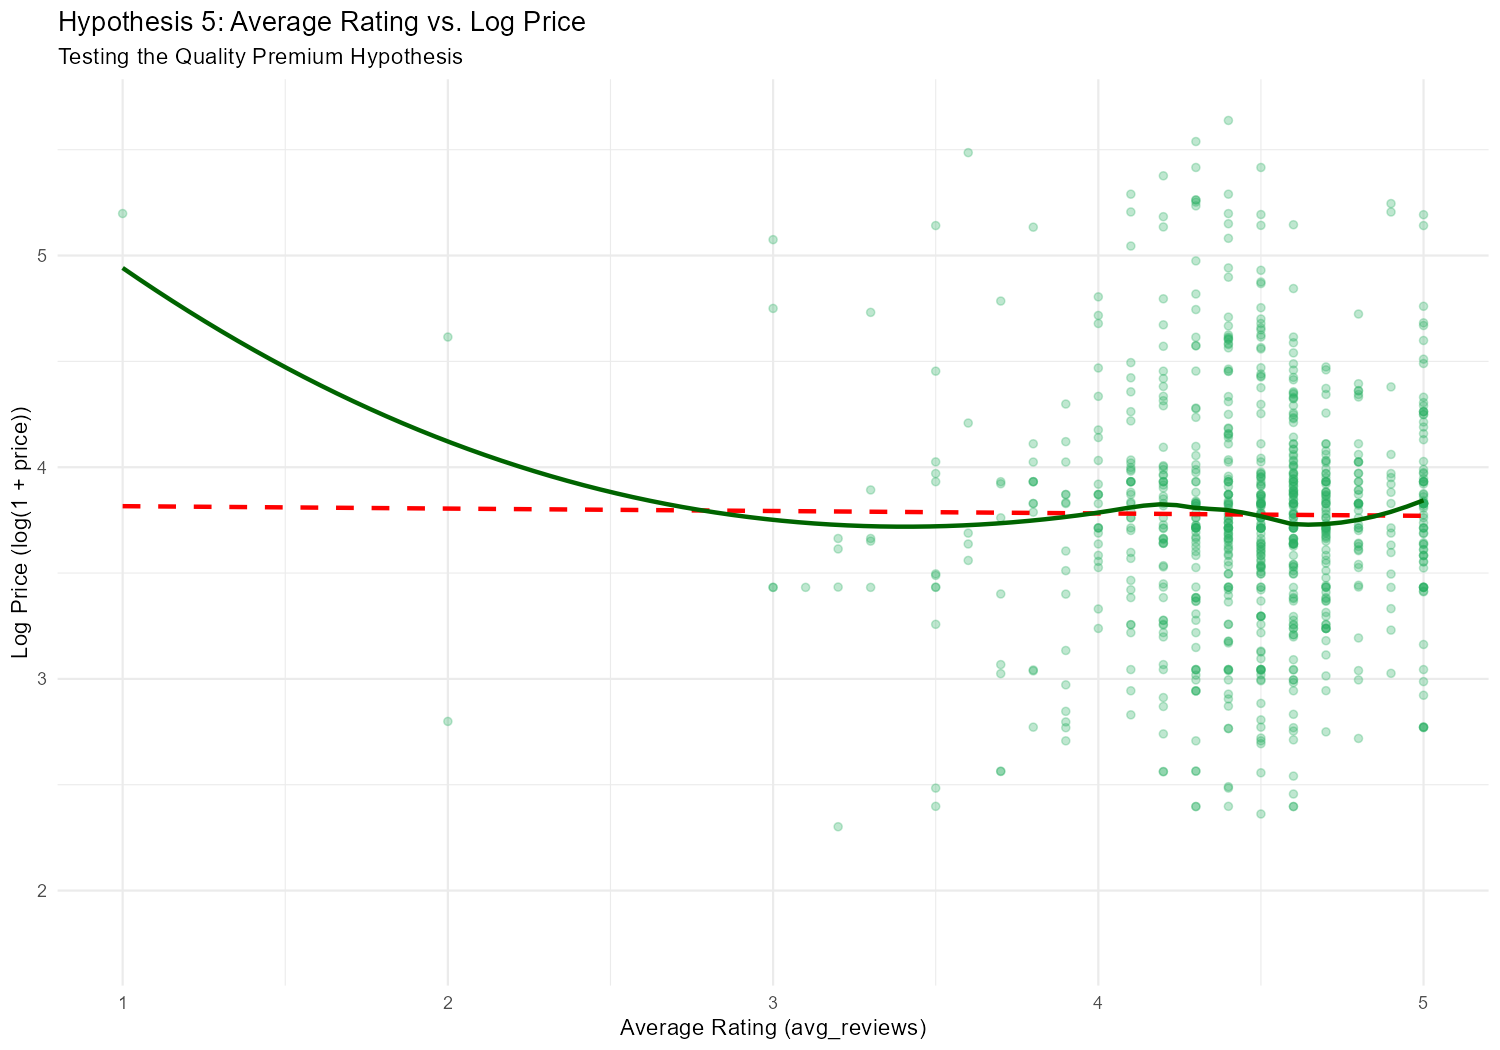
\includegraphics[width=0.85\textwidth]{plots/hypothesis_5_rating_price.png}
    \caption{Hypothesis 5: Relationship Between Average Customer Rating and Book Price}
    \label{fig:h5_plot}
\end{figure}

\subsubsection*{Empirical Results and Statistical Testing}

The Spearman rank correlation test revealed a negligible positive association between average customer ratings and log-transformed book price ($\rho = 0.01974$, $p = 0.5723$).

Since the p-value exceeds the conventional significance level of $\alpha = 0.05$, the null hypothesis cannot be rejected. The empirical findings suggest that average customer ratings do not exhibit a statistically significant monotonic association with book price.

% ==========================================
% 7. MULTIVARIATE MODELING
% ==========================================

\newpage
\section{Multivariate Econometric Modeling and Diagnostic Evaluation}

\subsection{Multiple Linear Regression Model}

To investigate the joint association between book characteristics and retail prices, a multivariate Ordinary Least Squares (OLS) regression model was estimated. The dependent variable was the log-transformed book price, while the independent variables included page count, review availability, and log-transformed review volume.

The econometric specification is expressed as:

\begin{equation}
\log(1+\text{price}_i)
=
\beta_0
+
\beta_1\text{pages}_i
+
\beta_2\text{has\_reviews}_i
+
\beta_3\log(1+\text{n\_reviews}_i)
+
\varepsilon_i
\end{equation}

where $\beta_0$ represents the intercept, $\beta_1$, $\beta_2$, and $\beta_3$ represent the regression coefficients, and $\varepsilon_i$ denotes the error term.

\subsection{Empirical Regression Results}

The estimated model was statistically significant, with an overall F-statistic of $F(3,926)=127.6$ and a p-value below $2.2 \times 10^{-16}$.

The model achieved an $R^2$ of approximately $0.2924$ and an adjusted $R^2$ of $0.2901$, indicating that approximately 29\% of the variation in log-transformed book prices is explained by the included predictors.

\begin{table}[htbp]
\centering
\caption{OLS Regression Results}
\label{tab:ols_results}
\begin{tabular}{lrrr}
\toprule
Variable & Coefficient & t-value & p-value \\
\midrule
Pages & 0.001507 & 18.976 & $< 2 \times 10^{-16}$ \\
Has Reviews & 0.005236 & 0.086 & 0.931 \\
Log Review Count & -0.072204 & -6.771 & $2.27 \times 10^{-11}$ \\
\bottomrule
\end{tabular}
\end{table}

\subsection{Interpretation of Regression Coefficients}

The page count coefficient is positive and highly statistically significant ($\beta_1=0.001507$, $p<0.001$), suggesting that longer books tend to have higher prices, holding the other included variables constant.

The review availability indicator is not statistically significant ($\beta_2=0.005236$, $p=0.931$), suggesting that the presence of reviews does not independently explain price differences after controlling for page count and review volume.

Conversely, log-transformed review volume exhibits a statistically significant negative coefficient ($\beta_3=-0.072204$, $p<0.001$), indicating that books with greater review engagement tend to have lower prices, conditional on the other variables.

\subsection{Multicollinearity Assessment}

Variance Inflation Factors (VIF) were calculated to evaluate potential multicollinearity among the independent variables.

\begin{table}[htbp]
\centering
\caption{Variance Inflation Factors}
\label{tab:vif_results}
\begin{tabular}{lr}
\toprule
Predictor & VIF \\
\midrule
Pages & 1.0458 \\
Has Reviews & 1.6429 \\
Log Review Count & 1.6967 \\
\bottomrule
\end{tabular}
\end{table}

All VIF values are substantially below the conventional threshold of 5, suggesting that severe multicollinearity is not present among the selected predictors.

\subsection{Regression Diagnostic Evaluation}

Regression diagnostic plots were examined to evaluate the behavior of model residuals, identify potentially influential observations, and assess the suitability of the OLS specification.

\begin{figure}[H]
    \centering
    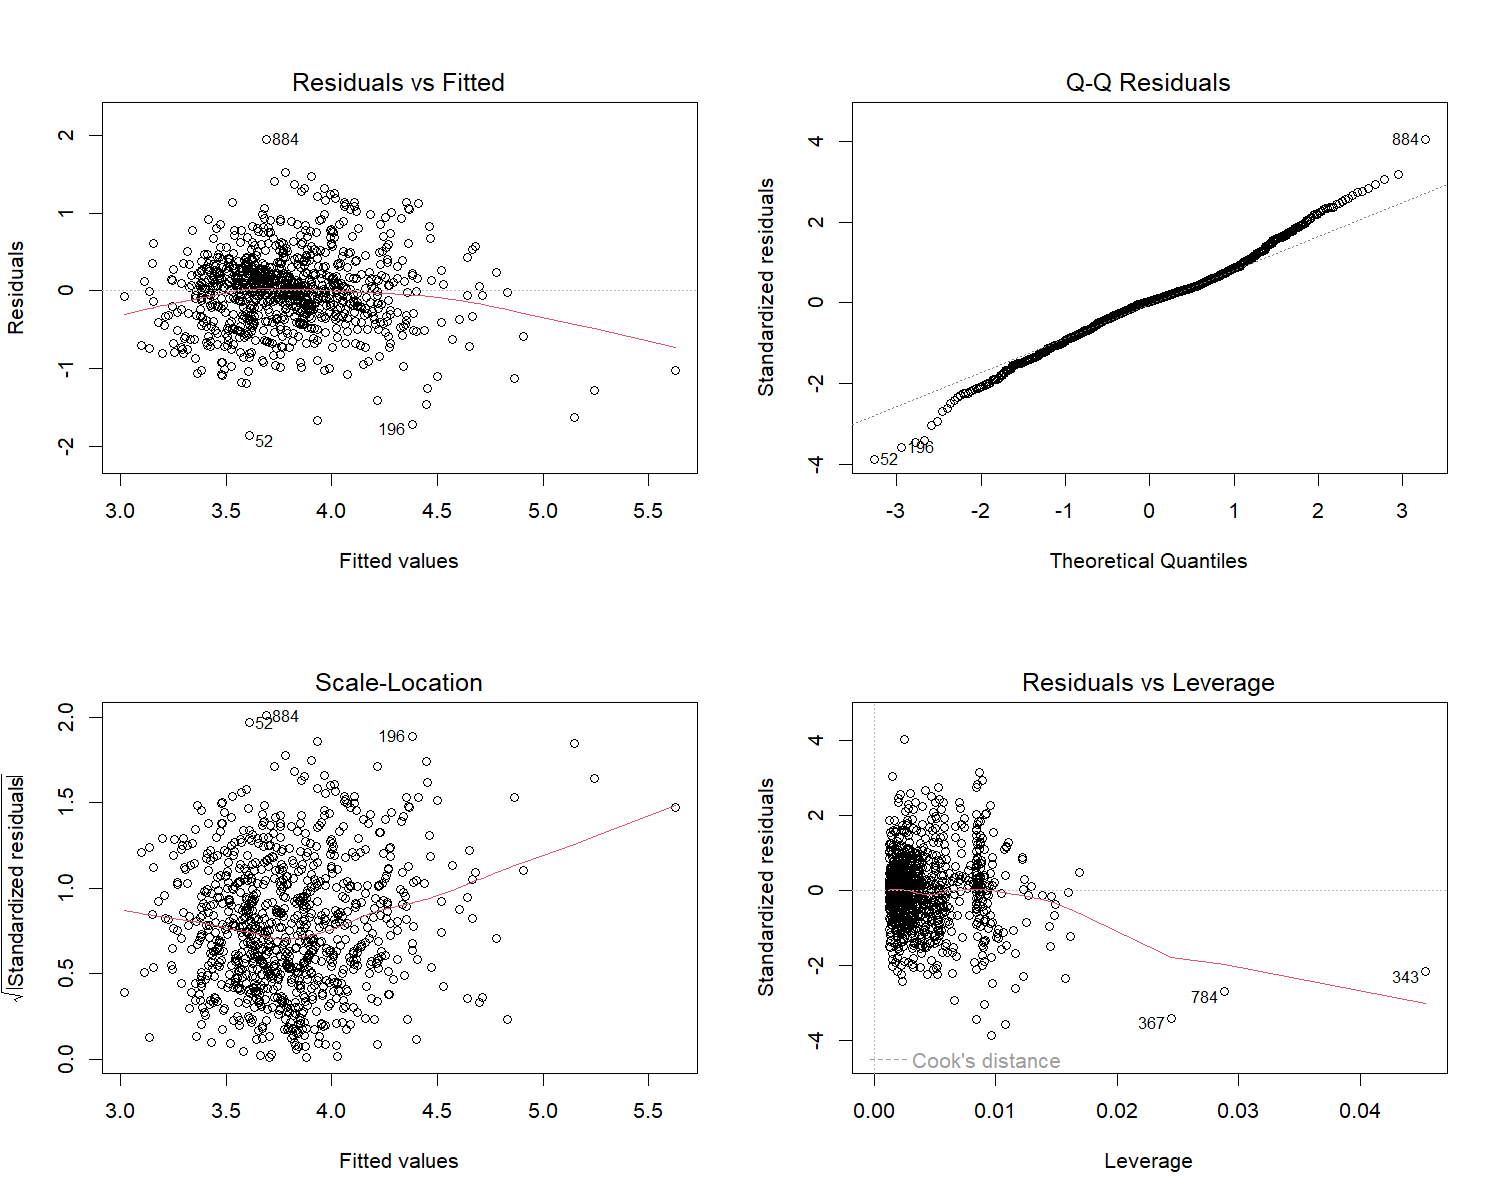
\includegraphics[width=0.95\textwidth]{plots/ols_model_diagnostics.png}
    \caption{OLS Regression Diagnostic Plots}
    \label{fig:ols_diagnostics}
\end{figure}
\newpage
\subsubsection*{Assessment of OLS Diagnostic Plots}

\begin{enumerate}
    \item \textbf{Residuals vs Fitted (Linearity):}
    The residuals are generally centered around zero,
    although mild curvature suggests possible deviations
    from the linearity assumption.

    \item \textbf{Normal Q-Q Plot (Normality):}
    The residuals approximately follow the theoretical
    quantiles in the central region, but deviations
    in the tails suggest departures from normality.

    \item \textbf{Scale-Location Plot (Homoskedasticity):}
    The upward trend in residual spread at higher fitted
    values suggests possible heteroskedasticity.
    Therefore, constant error variance cannot be
    confidently assumed.

    \item \textbf{Residuals vs Leverage (Influence):}
    Some observations exhibit relatively higher leverage
    or residual values and may warrant further
    investigation. The diagnostic plot alone does not
    establish the absence of influential observations.
\end{enumerate}
Overall, the diagnostic plots suggest that some OLS
assumptions may not be fully satisfied. Consequently,
the regression results should be interpreted with
appropriate caution.

\end{document}

